\chapter{Разработка архитектуры модульной платформы технологического оборудования}\label{ch:ch2}

\section{Общие положения}

Адаптивная платформа технологического оборудования (\textit{ADAPTEQ}, сокр.~от~англ. \textit{ADAptive Platform of Technological EQuipment}) является программно-аппаратным комплексом для создания различных видов промышленного оборудования с числовым программным управлением. Основа ADAPTEQ "--- шасси универсальное трехкоодинатное (сокр. \textit{ШУТ}), которое играет роль механизма перемещения рабочих органов, определяющих тип оборудования. Связь с персональным компьютером и~генерация управляющих сигналов для исполнительных и рабочих органов шасси осуществляется с помощью управляющего блока.

Для подготовки управляющих программ используется совокупность программных средств с открытым исходным кодом, именуемая TAPS (сокр.~от~англ. \textit{Technological Automation Python based System} "--- Автоматизированная Технологическая Система на базе Python). TAPS представляет собой интерфейс обмена данными между различными пакетами прикладных программ технологического назначения, созданный на языке программирования Python.

Очевидно, что область применения TAPS может быть гораздо шире, чем просто подготовка управляющих программ для ШУТ, с ее помощь возможна практически бесшовная интеграция и передача всех данных о~проектируемом (разрабатываемом, изготавливаемом, прототипируемом, исследуемом и~т.\:д.) изделии на всех этапах его жизненного цикла.

Таким образом, ADAPTEQ можно представить как совокупность двух неизменных частей (ШУТ и универсальный блок управления) и двух параметризуемых частей (рабочий орган и программное обеспечение).

Двумя основными постулатами концепции ADAPTEQ являются \textit{унификация} и \textit{гибридизация}. Под унификацией понимаются открытые программная и аппаратная архитектуры, позволяющие создавать новые типы оборудования и программного обеспечения для работы с ним по принципу <<интеллектуального конструктора>>.

Унификация достигается за счёт разбиения единого изделия на крупные, взаимозаменяемые блоки с чётким описанием входных и~выходных параметров каждого блока.

Первый блок "--- это \textit{ШУТ}, для него должны быть четко прописаны габаритные размеры рабочей области, посадочные места для крепления рабочих органов, механические и электрические характеристики приводов.

Второй блок "--- \textit{универсальный} \textit{блок управления}. Для универсального блока управления должны быть стандартизованы электрические соединители, позволяющие подключать к~нему ШУТ и вспомогательные блоки, сигналы (протоколы), помощью которых осуществляется управление, внутреннее и внешнее представление управляющей программы, параметры и протокол связи с персональным компьютером.

Третий блок "--- \textit{рабочий орган}, т.е. сопрягаемое с ШУТ и блоком управления устройство, которое определяет назначение оборудования. Для него должны быть стандартизованы максимальные габаритные размеры, посадочные места, а также способ сопряжения с блоком управления. Рабочий орган "--- наиболее сложная часть всей концепции, поэтому он требует наиболее полного описания и стандартизации.

На рабочий орган должны быть наложены определенные ограничения, позволяющие абсолютно точно сказать, что спроектированный на его основе модуль сможет беспрепятственно быть интегрирован с ШУТ и блоком управления. К таким ограничениям можно отнести, например, следующие: максимальная масса, напряжение питания, количество и мощность используемых шаговых или серводвигателей и~т.\:д.

Замена рабочего органа позволит создавать на базе концепции \foreignlanguage{english}{ADAPTEQ} следующие виды оборудования:
\begin{itemize}
	\item Фрезерные станки.
	
	\item Граверы.
	
	\item Лазерные резаки.
	
	\item 3\foreignlanguage{english}{D-}принтеры.
	
	\item Контрольно-измерительные машины.
	
	\item Машины для установки компонентов на печатную плату.
	
	\item Маркировщики.
	
	\item Сортировщики.
	
	\item Дозаторы химических реактивов.
	
	\item Декартовые роботы.
	
	
\end{itemize}
Четвертый блок "--- \textit{программное обеспечение}, унификация которого осуществляется за счет универсального интерфейса между TAPS и~внутренним программным обеспечением блока управления (<<прошивок>> микроконтроллера).

Гибридизация ADAPTEQ является прямым следствие унификации, так как использование унифицированных и сопрягаемых между собой модулей позволяет создавать новые виды оборудования, являющиеся совокупностью существующих. Например, можно создать аддитивно-субстрактивную установку быстрого прототипирования, сочетающую в~себе характеристики 3D-принтера и трёхкоодинатного фрезерного станка или совместить фрезерную головку для черновой обработки заготовок с~лазером для полирования определенных поверхностей.

Для этого на базе спецификации и ограничений рабочего органа могут быть созданы гибридные фрезерно-печатающие или фрезерно-полирующие головки, а также гибридное программное обеспечение, работающее с одной и той же трехмерной моделью вначале для послойного разбиения, а затем для селективной доработки некоторых поверхностей напечатанного изделия фрезером (лазером).

\textbf{2.2. Обоснование необходимости создания ADAPTEQ}

В последние годы в России появляется все больше малых инновационных предприятий. Малые инновационные предприятия (МИП) являются одним из видов структуры новаторского типа, которая получила название стартап (англ. \textit{start-up}).

Особенностью такого предприятия является нацеленность на производство конкретной продукции. В связи с новизной такого вида структур, пока не сформировалось однозначное представление о том, что такое малое инновационное предприятие. До сих пор оно определяется как предприятие, разрабатывающее и внедряющее в производство наукоемкие технологии и изделия. Такое определение является слишком общим и не затрагивает ключевые особенности.

Более конкретно МИП описывает следующее определение: малое инновационное предприятие "--- это объединение специалистов, имеющих определенные знания, аппаратные и программные ресурсы для решения задач подготовки производства или непосредственного производства продукции.

Хотя в такой формулировке МИП и не описывается абсолютно конкретно с отсечением других схожих структур, также базирующихся на понятии стартап, но уже включает ряд характерных особенностей такого предприятия. Более точное определение можно дать только в рамках решаемых им задач. С этой точки зрения можно выделить три типа МИП:

\begin{itemize}
	\item Инжиниринговые центры.
	
	\item Малые производства.
	
	\item Fab lab\footnote{сокр.~от~англ. \textit{fabrication laboratory}, в данной работе при упоминании формаций, удовлетворяющих требованиям fab lab, также будет использоваться термин \textit{промлаб}, сокр. от \textit{промышленная лаборатория}.}.
	\end{itemize}

\textit{Инжиниринговые центры} представляют собой организации, выполняющие инжиниринговые услуги, то есть комплекс коммерческих услуг по подготовке и обеспечению процесса производства и реализации продукции, по обслуживанию и эксплуатации промышленных, инфраструктурных и других объектов.

Формирование инжиниринговых центров производится на базе тех ресурсов, которые не задействованы в производственном процессе, задействованы не полностью или не предназначены для производства продукции. Таким образом, инжиниринговые центры формируются на базе предприятий или учебных заведений с подготовленной базой современного оборудования. В таком виде МИП специализируется на предоставлении услуг в соответствии с~имеющимися у них компетенциями.

Другим подходом является использование схемы MiP (сокр.~от~англ. \textit{Mini Production} "--- малое производство), соответствующей типу <<Малое производство>>, когда основной целью МИП является выпуск продукции, которая может быть использована как конечным пользователем, так и~другими предприятиями при производстве своей продукции.

Для MiP на текущем этапе развития характерна некоторая спонтанность организации без единых принципов развития, свойственных всем представителям этого направления. Однако можно выделить ряд критериев, позволяющих называть такие компании предприятиями, и характеризующие их как перспективные и стабильные за счет проработанной стратегии развития.

Последний вид МИП, \textit{промлаб}, является небольшой мастерской коллективного пользования, предоставляющей всем участникам данного предприятия доступ к различному высокотехнологичному оборудованию. Как правило, промлаб располагают набором средств, позволяющим выпускать различные инновационные продукты, в том числе и мелкими сериями. 

Очевидно, что для создания МИП любого из перечисленных типов необходимо большое количество разнообразного, зачастую очень дорогого, технологического оборудования. В то же время задачи, решаемые в рамках МИП, не требуют высокой точности или производительности, присущей профессиональным образцам подобного оборудования, но для многих типов оборудования найти менее точные или производительные аналоги просто не представляется возможным.

Следует также отметить, что одной из ключевых характеристик МИП является их универсальность. При этом универсальность проявляется не столько в выпускаемой продукции (хотя и в этой области МИП обязано быть достаточно гибкой структурой), сколько в используемых средствах и навыках специалистов. Таким образом, унификация решаемых задач в рамках одного устройства является важным преимуществом для производственных МИП.

ADAPTEQ призвана стать решением вышеописанных задач, так как является модульной, унифицированной и легко переналаживаемой платформой, на основе которой, путем простого добавления или замены одного или нескольких компонентов, может быть создано то или иное устройство. Например, заменой рабочего органа можно из фрезерного станка получить установку быстрого прототипирования (также обозначаемую как 3D-принтер), координатно-измерительную машину (сокр. \textit{КИМ}) или другое устройство портального типа.

Однако замены рабочей части устройства и подключения всех коммуникаций недостаточно, так как для разных устройств используется различный способ управления, что требует различных подходов в проектирование программного обеспечения. Так, фрезерный станок требует определения областей обработки с последующим формированием G-кода и его трансляции в инструкции для системы перемещения. Работа с установкой быстрого прототипирования имеет схожий принцип, только вместо областей обработки в качестве отправной информации используется геометрия выращиваемого слоя со структурами поддержки. С другой стороны КИМ должны работать как в автоматическом режиме, движения в котором аналогичны таковым для фрезерного станка, так и в ручном режиме, требующем точного выполнения инструкций оператора, что требует унификации и программного обеспечения тоже, что является одной из основных особенностей предлагаемой концепции ADAPTEQ.

\textbf{2.3 Аналоги предлагаемой концепции}

Прямых аналогов предлагаемой концепции адаптивной платформы технологического оборудования авторами найдено не было, поэтому будут рассмотрены проекты и готовые продукты, сходные с ADAPTEQ по тем или иным параметрам, первым из которых является \textit{универсальность рабочего органа}, то есть возможность путём простой переналадки менять тип оборудования. 

На сегодняшний день на рынке представлены несколько типов универсальных модульных настольных станков нижнего ценового диапазона. Одним из наиболее известных производителей подобного оборудования является компания \textit{Proxxon}~(рисунок~\cref{fig:proxxon}), выпускающая различные настольные станки <<хоббийного>> класса, в основном токарно-фрезерно-сверлильной группы, распиловочное оборудование и ручной электроинструмент. Большое количество универсальной оснастки и~взаимозаменяемость многих частей оборудования Proxxon позволяет использовать его в небольших мастерских, а также на малых инновационных предприятиях, но с рядом ограничений:

\begin{itemize}
	\item В базовой комплектации все оборудование ручное. Возможность переделки под числовое программное управление (ЧПУ) является опцией. Возможности ЧПУ сильно ограничены.
	
	\item Спецификации оборудования закрыты, создание своих модулей невозможно, либо возможно, но только с~применением реверс-инжиниринга.
	
	\item Как уже было отмечено выше, все оборудование Proxxon субстрактивного типа, возможность использовать его для создания 3d-принтера или контрольно-измерительной машины отсутствуют, так как нет единой модульной структуры блока управления ЧПУ, а также фирменного программного обеспечения.	
\end{itemize}

\begin{figure}[ht]
	\centerfloat{
		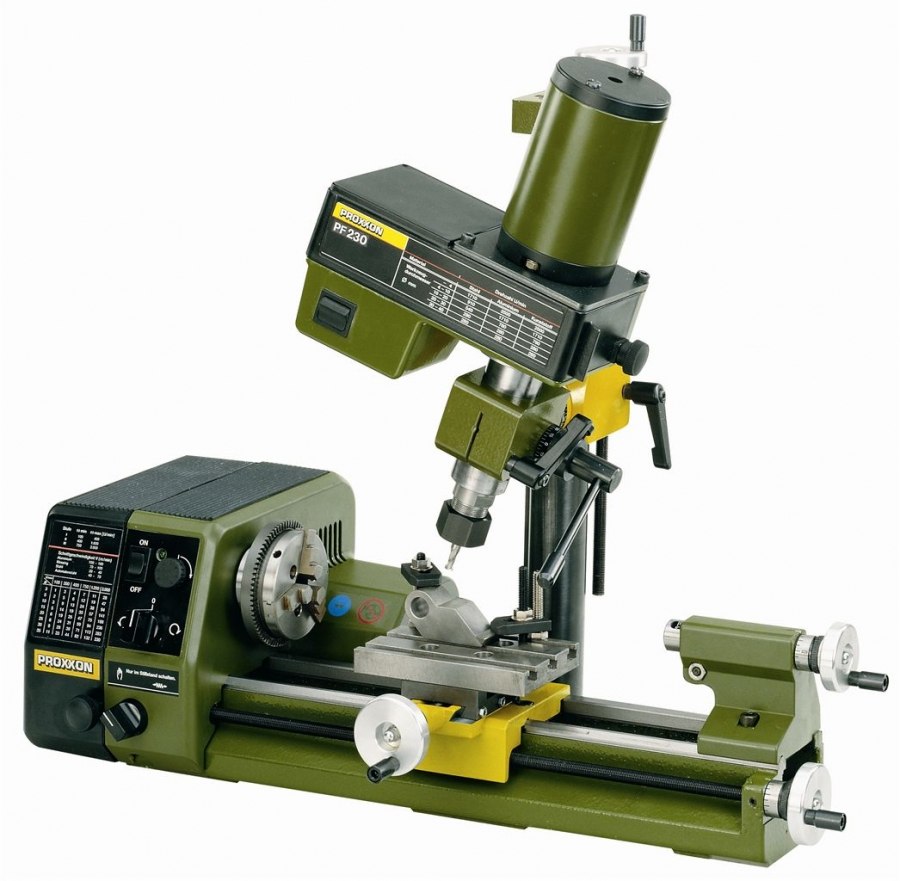
\includegraphics[scale=0.27]{ch-2/image1.png}
	}
	\caption{Пример оборудования компании Proxxon.}\label{fig:proxxon}
\end{figure}

Стоит также отметить настольные модульные универсальные станки, выпускаемый немецкой компанией TheCoolTool (thecooltool.com), в~особенности модели UNIMAT~1~(рисунок~\cref{fig:unimat-2}) и UNIMAT CNC~(рисунок~\cref{fig:unimat-2}).

\begin{figure}[ht]
	\centerfloat{
		\hfill
		\subcaptionbox{\label{fig:unimat-1}}{%
			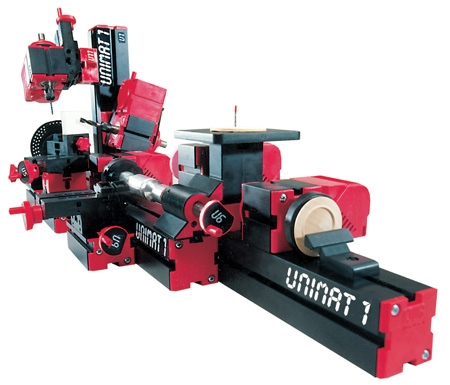
\includegraphics[width=0.4\linewidth]{ch-2/image2}}
		\hfill
		\subcaptionbox{\label{fig:unimat-2}}{%
			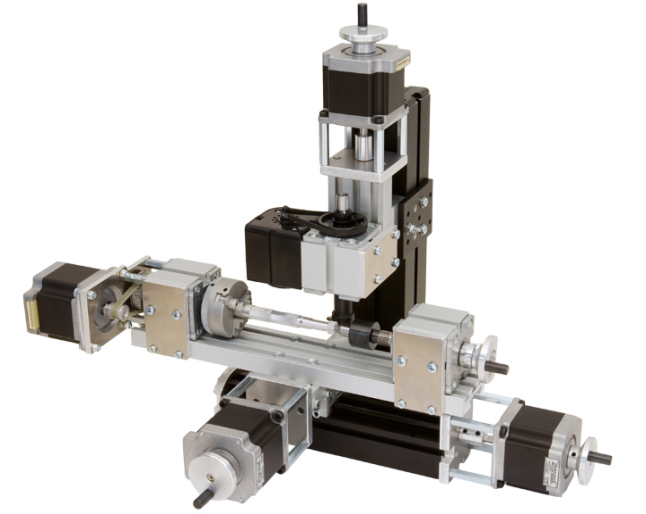
\includegraphics[width=0.4\linewidth]{ch-2/image3}}
		\hfill
	}
	\caption{Настольные модульные станки UNIMAT 1 (\textit{а}) и UNIMAT CNC (б).}\label{fig:unimat}
\end{figure}

Первый из рассматриваемых станков представляет собой модульную систему <<6 в 1>> с ручным управлением (переделка под ЧПУ возможна только с применением специальных доработок и реверс-инжиниринга), то есть позволяет в зависимости от компоновки модулей производить:
\begin{itemize}
	\item Распиловку деревянных и металлических заготовок вертикально расположенным ножовочным полотном.
	
	\item Токарную обработку деревянных заготовок.
	
	\item Токарную обработку металлических заготовок.
	
	\item Плоское торцевое шлифование с возможностью снятия шлифовального блока для ручной обработки шлифовальным кругом.
	
	\item Вертикальное и горизонтальное фрезерование.
	
	\item Сверление с возможностью поворота сверлильной головки на 360$^{\circ}$ или снятия её для ручного сверления.
	
	
\end{itemize}
Возможность совмещения двух операций без переналадки оборудования отсутствует.

Второй является токарно-фрезерно-сверлильным модульным станком с ЧПУ, в котором в зависимости от компоновки существует возможность управления шестью осями одновременно, что позволяет совмещать операции обработки без перенастройки модулей. Достоинством данного оборудования является большая открытость программной архитектуры, что подтверждается возможностью использовать для управления осями станка не только фирменное закрытое программное обеспечения, но и открытое решение EMC2, построенное на базе свободной операционной системы Linux. При этом сам станок представляет собой лишь набор управляемых электроприводов без внутреннего блока управления, что требует постоянного подключения к персональному компьютеру, приобретаемому отдельно.

К недостаткам можно отнести:
\begin{itemize}
	\item закрытую аппаратную архитектуру рассматриваемого продукта, что существенно усложнит переделку данного решение подо что-то отличное от металлообрабатывающих станков;
	
	\item неудачную геометрическую компоновку станка, что также ставит по сомнение возможность его переделки под другие нужды (например, очевидно, что подобная кинематическая схема вряд ли позволит использовать ее в качестве трёхмерного принтера или контрольно-измерительной машины);
	
	\item отсутствие портала, что влечет за собой снижение жёсткости связки координатных осей, а, следовательно, и жесткости станка в целом. Последнее будет особенно заметно при максимально удалении осей, из-за чего может пострадать точность обработки. Данное предположение подтверждается спецификациями, размещенными на сайте производителя, где указывается, что точность установки не может превысить 80мкм.
	
	\item низкую мощность приводов осей, а также очень небольшие рабочие ходы по некоторым из них.
	
	
\end{itemize}
Из всего вышесказанного можно сделать вывод о том, что за исключением возможности использования свободного программного обеспечения рассматриваемый продукт не удовлетворяет требованиям концепции ADAPTEQ и не может быть рассмотрен в качестве её прямого аналога.

Второй параметр, по которому проводилось сравнение предлагаемой концепции с существующими аналогами "--- \textit{открытая аппаратная архитектура}, позволяющая создавать новые типы оборудования без необходимости создания каких-то дополнительных переходных блоков и применения реверс-инжиниринга.

Для сравнения были рассмотрены два проекта, целью которых является создание открытой платформы универсального оборудования с ЧПУ:

\begin{enumerate}
	\item \foreignlanguage{english}{\textbf{Build Your Own CNC}} (\href{https://www.buildyourcnc.com/cnckit2.aspx}{\foreignlanguage{english}{buildyourcnc.com}}).
	
	\item \textbf{Shapeoko} (shapeoko.com).
\end{enumerate}

Рассмотрим оба этих проекта более подробно. \textit{Build Your Own CNC}~(рисунок~\cref{fig:byocnc}) "--- коммерческий проект по созданию универсального сборного оборудования с числовым программным управлением. Может считаться условно открытым, так как с одной стороны на сайте производителя отсутствуют чертежи и прочая техническая документация, необходимая для самостоятельного изготовления того или модуля оборудования (за исключением файлов раскроя основных корпусных деталей), но с другой стороны компания принимает запросы от пользователей на создание новых модулей (новых типов оборудования). Финансирование данных исследований проводится за счёт средств, полученных в качестве пожертвований от пользователей, а также за счет основного бизнеса компании "--- производства и продажи модулей и готовых сборных устройств.

На сегодняшний день в рамках проекта \textit{Build Your Own CNC} реализовано достаточно большое количество модулей и готовых устройств среди которых можно выделить:

\begin{itemize}
	\item Установку для лазерной резки и гравирования.
	
	\item Трёхкоординатное фрезерные и сверлильные станки различных компоновок и типоразмеров с множеством сменных головок, среди которых необходимо выделить печатающую головку, позволяющую создать на основе предлагаемой платформы 3d-принтер типа FDM\footnote{сокр.~от~англ. \textit{Fused Deposition Modeling} "--- моделирование методом наплавления.}.
\end{itemize}

\begin{figure}[ht]
	\centerfloat{
		\hfill
		\subcaptionbox{\label{fig:byocnc-1}}{%
			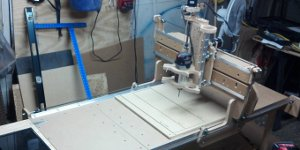
\includegraphics[width=0.7\linewidth]{ch-2/image4}}
		\hfill
		\subcaptionbox{\label{fig:byocnc-2}}{%
			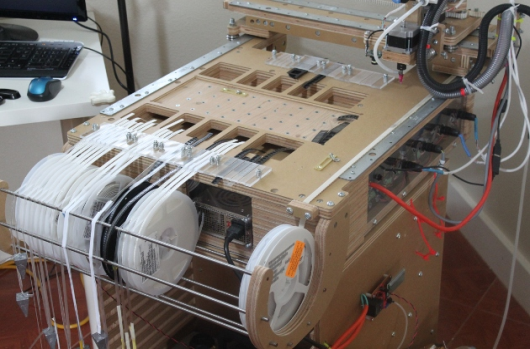
\includegraphics[width=0.7\linewidth]{ch-2/image5}}
		\hfill
	}
	\caption[Примеры оборудования, созданного в рамках проекта \textit{Build Your Own CNC}]%
		{Примеры оборудования, созданного в рамках проекта \textit{Build Your Own CNC}: фрезерный станок портального типа (\textit{а}), установка для позиционирования электронных компонентов на печатной плате (\textit{б}).}\label{fig:byocnc}
\end{figure}


\begin{itemize}
	\item Распиловочные вертикальные станки.
	
	\item Установку для автоматического размещения электронных компонентов на печатной плате (англ. \textit{Pick and Place machine}).
	
	
\end{itemize}
В планах компании также разработать:
\begin{itemize}
	\item Пятикоординатный фрезерный станок.
	
	\item 3d-принтер, использующий технологию фотолитографии.
	
	\item 3d-принтер, использующий технологию селективного лазерного спекания.
	
	\item Станки токарной группы.
	
	\item 3d-сканер.
	
	
\end{itemize}
К недостаткам данного проекта можно отнести следующие:
\begin{itemize}
	\item Как уже отмечалось ранее, проект не является полностью открытым с точки зрения аппаратного обеспечения.
	
	\item На текущий момент реализовано очень малое количество типов оборудования. Отчасти это связано с первым недостатком, так как спецификации закрыты и разработкой новых модулей и типов оборудования занимаются только сотрудники компании.
	
	\item Отсутствует единая универсальная кинематическая схема, из-за чего для каждого нового вида оборудования необходимо проектирование новой кинематической схемы, а также сопутствующие этому процессу расчеты и моделирование.
	
	\item Отсутствует единый подход к проектированию линейных приводов. Предполагается возможность использования как ходовых винтов с трапециевидной резьбой, так и передач на основе зубчатых ремней и цепей. Особо настораживает использование цепных передач в прецизионных настольных станках для установки электронных компонентов на плату.
	
	\item Основной материал, из которого изготавливаются все несущие и корпусные детали всех видов оборудования "--- клеевая фанера. При всех очевидных достоинствах данного материала таких, как легкость обработки, хорошее виброгашение, высокая прочность, низкая цена, целесообразность использования данного материала для создания высокоточного оборудования с ЧПУ вызывает большие сомнения. Очевидно, что авторам проекта вряд ли удалось достичь высокой жесткости конструкции и точность оборудования оставляет желать лучшего.
	
	\item Привода всех модулей и всех типов готового оборудования не имеют никаких датчиков обратной связи по положению. Авторы проекта исходят из предположения, что используемые ими шаговые двигатели никогда не пропускаю шагов, драйверы шаговых двигателей всегда генерируют правильную последовательность импульсов, а используемые кинематические схемы не подвержены заклиниванию.
	
	\item Компания не занимается производством или разработкой блоков управления для своего оборудования и вообще каких-либо электронных или электрических компонентов. Клиентам предлагаются готовые силовые блоки сторонних фирм, а~управление отдается либо на откуп персонального компьютера, либо известной платформе разработки и отладки электроники Arduino.
	
	\item Также компания не занимается разработкой программного обеспечения для своего оборудования. Пользователям предлагается воспользоваться либо уже упоминавшимся ранее открытым пакетом EMC2, либо приобрести одно из многочисленных коммерческих решений с тем же функционалом.
	
	\item Даже в проектах отсутствует какое-либо упоминание блока автоматической смены инструмента.
	
	
\end{itemize}
Второй проект, выбранный для анализа "--- \textit{Shapeoko}~(рисунок~\cref{fig:shapeoko}) является полностью открытым проектом по созданию трехкоординатной платформы портального типа. Из очевидных достоинств проекта можно выделить созданное авторами проекта программное обеспечение с открытым исходным кодом, а также полностью открытые спецификации аппаратной части, включающие в себя чертежи, трехмерные модели и прочую техническую документацию, необходимую для самостоятельной реализации разработанного авторами оборудования.

\begin{figure}[ht]
	\centerfloat{
		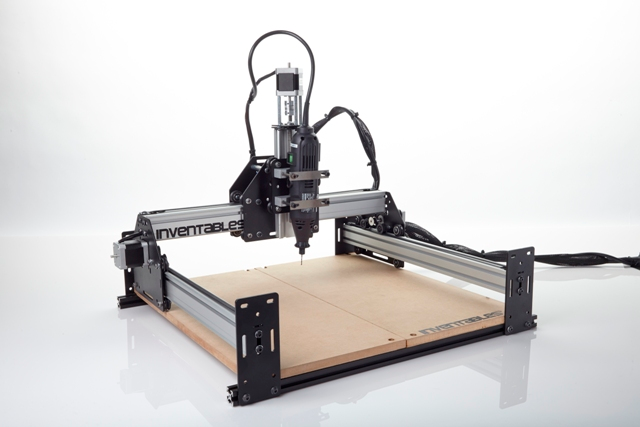
\includegraphics[scale=0.5]{ch-2/image6.png}
	}
	\caption{Трёхкоординатный фрезерный станок, реализованный в рамках открытого проекта \textit{Shapeoko}.}\label{fig:shapeoko}
\end{figure}

На данный момент проект находится на очень ранней стадии развития, поэтому не удалось провести детальный и всесторонний анализ недостатков представляемого проекта. Тем не менее, некоторые из них можно выделить уже сейчас:
\begin{itemize}
	\item Проект ориентирован в основном на трёхкоординатную фрезерную обработку и не позиционируется как модульная универсальная платформа.
	
	\item Управление опять отдается на откуп обычного персонального компьютера, за тем лишь исключением, что вместе пакета EMC2 авторы предлагают собственное программное обеспечение. О создании какой-либо модульной электронной системы управления речи не идет.
	
	\item Также как и в предыдущем проекте отсутствует какая-либо обратная связь по положению рабочего органа.
	
	\item Для передвижения портала использованы два шаговых двигателя, никак механически не синхронизированные между собой.
	
	\item Перемещение портала осуществляется за счёт зубчатых ремней, при этом не предусмотрены датчики обрыва ремня.
	
	\item Линейное перемещение всех координатных осей осуществляется за счет роликовых кареток. Сложность и~большое количество подвижных частей подобного механизма снижает надежность платформы. Также очевидно, что подобное решение может приводить к заклиниванию осей.
	
	\item В качестве основного и единственного на сегодняшний день рабочего органа используется гравер.
\end{itemize}

Последний параметр, выбранный для сравнения "--- \textit{модульная открытая архитектура блока управления} в совокупности с открытым исходным микрокодом электронного оборудования.

По данному параметру был найден единственный проект "--- анонсированный на 2015 год корпорацией Google модульный смартфон Ara. Безусловно, трудно производить сравнение модульной системы управления оборудования с ЧПУ и мобильную платформу для создания телефонов и планшетов, но такая цель и не ставилась.

Выбор был обусловлен уникальностью данного проекта. Подобные идеи звучали из уст представителей многих известных компаний и научных центров и ранее, но первая успешная попытка создать достаточно сложное электронное устройство из отдельных взаимозаменяемых модулей была сделана только сейчас. Очевидно, что это актуальное направление в ближайшее время получит свое развитие, также очевидно, что оно является очень перспективным и требует всестороннего исследования.

В силу своей специфики достоинства и недостатки проекта Ara рассматриваться не будут, вместо этого будет сделан обзор наиболее интересных и концептуальных решений, реализуемых в рамках данного проекта.

На официальном портале проекта корпорация Google заявляет, что разработала так называемый <<телефон-конструктор>> (рисунок~\cref{fig:ara}). Данный конструктор состоит из двух частей: эндоскелета (также часто называемого <<рамой>> и являющегося, по сути, внутренним каркасом) и~набора сменных модулей.

\begin{figure}[ht]
	\centerfloat{
		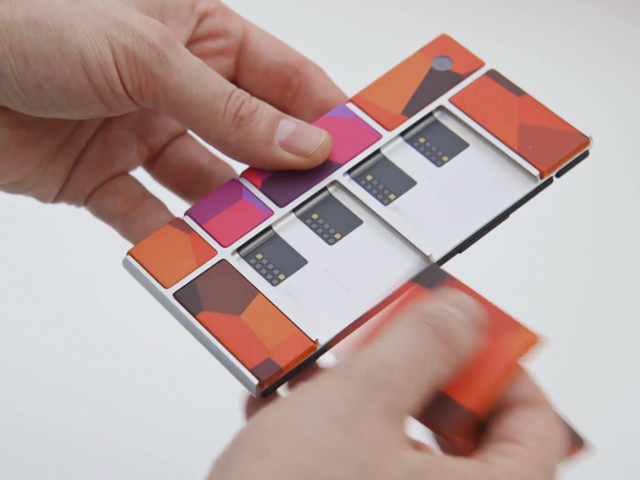
\includegraphics[scale=0.7]{ch-2/image7}
	}
	\caption{Модульный смартфон Ara.}\label{fig:ara}
\end{figure}

К эндоскелету могут быть подключены процессор со всей необходимой электрической <<обвязкой>>, жидкокристаллический дисплей, дополнительные модули оперативной памяти, физическая клавиатура, камера или дополнительный аккумулятор. Владелец телефон сможет сам производить модернизацию своего устройства или заменять поврежденные модули. Какие-то специальные инструменты или наличие каких-то знаний в области микроэлектроники или программирования не требуются.

Также за счет унификации габаритов эндоскелета и проектируемых модулей можно изменять размер аппарата, предполагается возможность создания как небольшого и очень компактного устройства, так и устройства, сравнимого по своим размерам с современными смартфонами и даже устройства больше похожего на интернет-планшет, а не мобильный телефон.

Очевидное достоинство подобного подхода для пользователя "--- возможность подбирать модули в соответствии со своими потребностями и финансовыми возможностями. Специалисты компании Google говорят, что в минимальной комплектации модульный смартфон будет стоить порядка 50 долларов США, а в максимальной "--- до 500.

Платформа позиционируется как открытая, то есть любой сторонний разработчик, использую так называемый MDK (сокр.~от~англ. \textit{Module Developers Kit} "--- набор инструментальных средств разработчика для создания модулей), сможет выпустить свой модуль, совместимый с Ara.

В спецификации говорится, что некоторые модули могут поддерживать так называемую <<горячую замену>>, то есть возможность сменить модуль без отключения питания аппарата. Также оговорен унифицированный способ крепления модулей к эндоскелету "--- крепление будет осуществляться за счет постоянных магнитов.

Каждый модуль может сочетать в себе несколько различных функций, например, можно создать гибридный модуль, являющийся экраном мобильного телефона и дополнительным аккумулятором, компенсирующим затраты энергии на подсветку и отображение информации.

Телефоны Ara будут работать под управлением операционной системы с открытым исходным кодом Android, что подтверждает полную программную и аппаратную открытость рассматриваемого проекта.

\textbf{2.4 Шасси универсальное трехкоординатное}

Шасси универсальное трехкоординатное представляет собой многоцелевую модульную систему, позволяющую создавать на своей основе различные типы высокотехнологичного оборудования, сопрягаемого с персональным компьютером. Конструктивно ШУТ является координатным столом портального типа с возможностью установки разнообразных рабочих органов (сменных модулей). Основными требованиями к ШУТ являются:

\begin{enumerate}
	\item Низкая себестоимость производства, достигаемая за счет модульности конструкции и использования недорогих стандартных комплектующих.
	
	\item Достаточная высокая точность позиционирования, достигаемая за счет использования датчиков обратной связи и простотой конструкции.
	
	\item Открытые программная и аппаратная архитектуры.
	
	\item Простота переналадки.
\end{enumerate}

Рассмотрим основные этапы проектирования ШУТ.

\textbf{2.4.1. Выбор компоновки и кинематической схемы ШУТ}

Для реализации ШУТ необходимо было сделать выбор базовой кинематической схемы, ведь именно она определяет основные механические и точностные характеристики будущего оборудования, построенного на базе предлагаемой платформы.

Первой из рассматриваемых стала так называемая платформа Стюарта~(рисунок~\cref{fig:stuart} представляет собой механизм с параллельной кинематикой, состоящий из шести пневматических, гидравлических или электрических линейных приводов. Данные приводы попарно размещаются на основании платформы, соединяясь (опять же попарно) в трех точках на верхней плите, повернутой на~\SI{120}{\degree} по отношению к нижней.

\begin{figure}[ht]
	\centerfloat{
		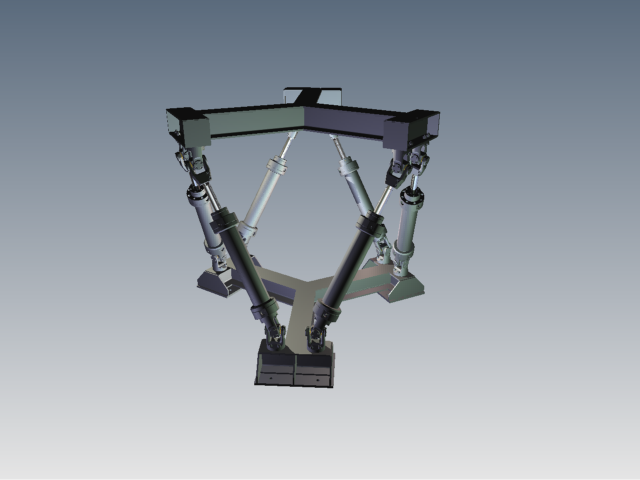
\includegraphics[scale=0.8]{ch-2/image8}
	}
	\caption{Пример платформы Стюарта.}\label{fig:stuart}
\end{figure}

Исполнительное устройство или рабочий орган размещаются на верхней плите и в определенном диапазоне линейных и угловых перемещений имеют шесть степеней свободы: линейное перемещение по осям x, y и z, а также вращения вокруг этих осей (крен, тангаж и рысканье).

К основным достоинствам данной кинематической схемы можно отнести:
\begin{itemize}
	\item Уже упомянутые ранее \textit{шесть степеней свободы}. Подобная конструкция позволяет рабочему органу двигаться по любой трехмерной траектории, что, безусловно, очень важно при создании таких типов оборудования как фрезерные металлорежущие станки и контрольно-измерительные машины.
	
	\item \textit{Высокая точность перемещения и повторяемость}. В отличие от других систем позиционирования любое перемещение платформы Стюарта требует изменения положения всех линейных приводов, что позволяет автоматически компенсировать механические погрешности, так как люфт не накапливает в какой-то одной координате, и может быть программно скомпенсирован на следующем этапе перемещения.
	
	\item \textit{Высокая жесткость конструкции}. Платформа Стюарта обеспечивает очень высокую жесткость своих механических компонентов и всех движущихся частей: подшипников, сочленений и приводных винтов (если они есть). Эта особенность позволяет достичь очень высоких значений собственной частоты конструкции (порядка~\SI{500}{\hertz} на~\SI{10}{\kilogram} нагрузки). Последнее означает, что построенные на базе платформы Стюарта металлорежущие станки могут работать на очень высоких скоростях резания. Кроме того, высокая жесткость конструкции дает возможность предотвратить изгиб линейных приводов, обеспечивающих движение платформы.
	
	\item \textit{Большая масса рабочего органа}. Вес рабочего органа, размещенного на верхней плите платформы Стюарта, равномерно распределен на шесть параллельных стоек. Это означает, что каждая из них несет на себе всего лишь одну шестую общего веса. Кроме того, каждая стойка работает только на растяжение и сжатие, не испытывая при этом никаких радиальных нагрузок. Следовательно, нет необходимости делать эти стойки массивными (как это делается в других подобных конструкциях).
	
	\item \textit{Большое разнообразие размеров платформы}. Конструктивные особенности платформы позволяют создавать на ее базе машине самых разных размеров в зависимости от целей и~задач, поставленных перед ними. По сравнению с другими подобными много осевыми конструкциями количество деталей, необходимых для создания платформы Стюарта на треть меньше, что делает конструкцию легче и подвижнее.
	
	
\end{itemize}
Несмотря на все вышеописанные достоинства, платформа Стюарта не лишена недостатков. Перечислим наиболее значимые из них:
\begin{itemize}
	\item \textit{Высокое трение}. Трение в многочисленных шарнирах "--- основной недостаток платформы Стюарта. Коэффициент трения конструкции равен примерно~0,8. Этого достаточно для небольшого осевого изгиба стоек (из-за незначительного заклинивания механизма), который, безусловно, влияет на точность и повторяемость конструкции. Использование керамического покрытия шарниров и специальной смазки позволяет снизить коэффициент трения до 0,2, но это существенно удорожает конструкцию.
	
	\item Даже с обычными шарнирами \textit{платформа Стюарта является очень дорогой конструкцией}. Большая стоимость определяется необходимостью использования шести линейных приводов. Также требуется гораздо более сложная система управления, причем как в программном (для быстрого и точного перемещения рабочего органа требуется постоянный пересчет его координат и перевод их в систему координат платформы), так и в аппаратном (все эти расчеты необходимо производить в режиме реального времени, что влечет за собой необходимость использования специализированных цифровых процессоров сигналов и более производительных микроконтроллеров). 
	
	\item \textit{Длина стоек.} Длина опорных стоек напрямую влияет на точность исполнительного механизма. При увеличении длины точность резко уменьшается из-за возможности изгиба. Также, возвращаясь к предыдущему пункту, можно сказать, что чем длиннее стойки, тем более дорогими будут линейные приводы, обеспечивающие их перемещение, но увеличение рабочей области без увеличения длины стоек невозможно.
	
	\item \textit{Динамическое тепловое расширение}. Вне зависимости от типа на высоких скоростях неизбежно возникает нагревание линейных приводов стоек платформы. В процессе работы механизма все стойки работают синхронно, однако степень нагрузки каждой из них различается. Это ведет к неконтролируемому изменению длины стоек, что увеличивает случайную погрешность позиционирования и снижает его точность. Единственный способ борьбы с динамическим тепловым расширением "--- постоянный их мониторинг и прогнозирование теплового расширения каждой стойки в реальном времени с помощью конечноэлементного анализа с последующим вводом компенсирующих перемещений. Безусловно, это еще больше усложняет и удорожает конструкцию.
	
	\item \textit{Необходимость калибровки механизма}. Точность параллельного механизма зависит от множества характеристик, для платформы Стюарта существует порядка 100 различных параметров, которые должны быть учтены в процессе настройки и калибрования механизма прежде, чем он сможет точно позиционировать свой рабочий орган.
	
	
\end{itemize}

\begin{figure}[ht]
	\centerfloat{
		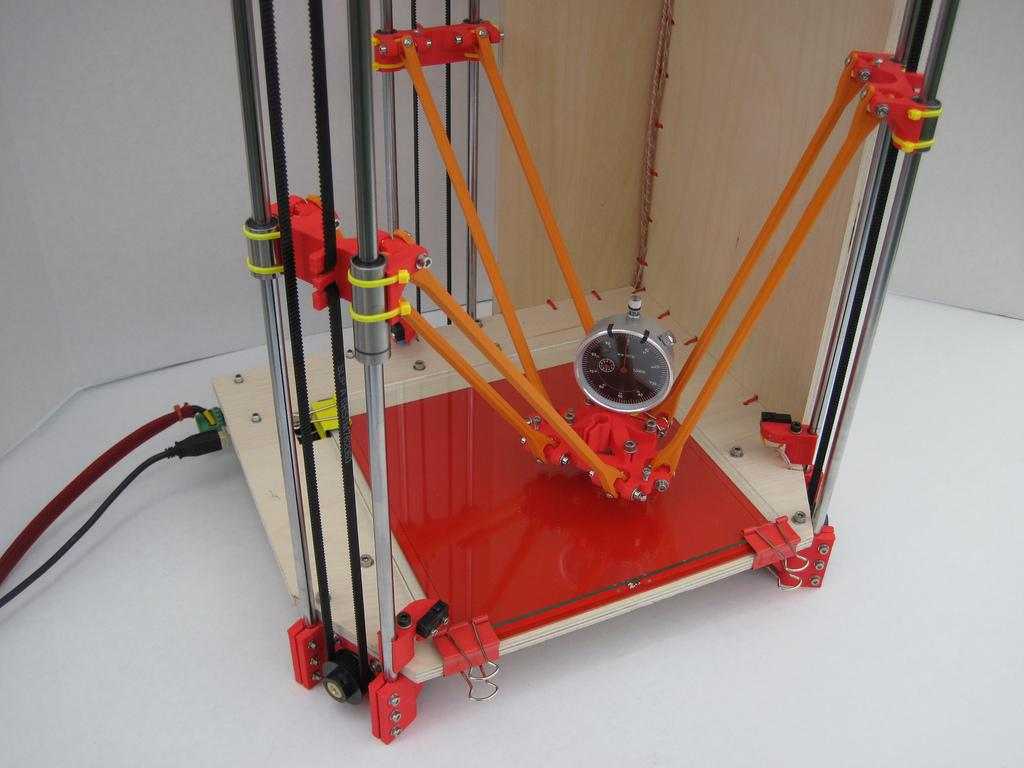
\includegraphics[scale=0.8]{ch-2/image9}
	}
	\caption{Дельта-робот.}\label{fig:delta}
\end{figure}

Помимо самой платформы Стюарта была также рассмотрена одна из ее разновидностей, а именно "--- дельта-робот~(рисунок~\cref{fig:delta}). Ключевой особенностью дельта-роботов является использование параллелограммов, положение которых задает перемещение рабочего органа дельта-робота.

В отличие от платформы Стюарта дельта-робот может позиционировать свой рабочий орган исключительно по трем основным координатам без вращений. Последнее существенно упрощает систему управления. Линейные приводы дельта-робота размещаются в~вертикальных стойках, что является его достоинством по сравнению с платформой Стюарта, так как линейные приводы не изменяют своей длины в процессе работы и подвержены минимальным осевым нагрузкам, что предотвращает их изгиб и позволяет увеличить жесткость конструкции.

Необходимо отметить, что рычажный механизм, связывающий каретки линейных приводов с креплением рабочего органа подвержен таким же нагрузкам, что и опоры платформы Стюарта, поэтому не исключен их изгиб под действием больших нагрузок. Единственный способ борьбы с этим явлением "--- увеличение массы стоек, что потребует существенного увеличения мощности линейных приводов и усложнения всей конструкции в целом. Также нельзя забывать, что рычаги соединяются с линейными приводами и креплением рабочего органа посредством цилиндрических шарниров (так как дельта-робот является разновидностью пантографа), надежность которых в жестких условиях эксплуатации является весьма сомнительной.

Как правило, рычаги делаются максимально легкими и жесткими за счет использования композиционных материалов, а сама конструкция чаще все находит применение в автоматических линиях, где требуется не высокая точность позиционирования, а большая скорость перемещения рабочего органа, которая для дельта-робота может достигать 10 м/с при ускорении до 30 g.

Из всего вышесказанного можно сделать вывод о том, что ни одна из рассмотренных разновидностей механизма с параллельной кинематикой не удовлетворяем всем требованиям, предъявляемым к ШУТ, поэтому перейдем к рассмотрению следующего класса механизмов пространственного перемещения "--- координатным столам.

Координатный стол представляет собой мехатронную систему, сочетающую в себе несущую конструкцию и механизм многоосевоей подачи, обеспеченной наличием нескольких пространственно расположенных линейных приводов. Как правило, координатные столы работают в декартовой системе координат, что в отличие от описанных ранее механизмов с параллельной кинематикой не требует постоянного пересчета координат перемещения рабочего органа.

В качестве несущей конструкции координатных столов может быть использована станина или рама, выполненные в виде сварного или литого каркаса из конструкционной стали (обычно используются качественные углеродистые стали, например, Сталь20 или Сталь40), также станина может быть отлита из чугуна (в большинстве случаев это серый чугун марок СЧ~15-32 и СЧ~18-36) или выполнена из полимерного бетона. Литая конструкция является более предпочтительной, однако используется только в случае, когда координатный стол будет эксплуатироваться в особо жестких условиях, например в высокоскоростных металлорежущих станках, в остальных случаях чаще применяется сварная рама из стали.

Основное назначение станины "--- обеспечение жесткости конструкции стола и гашение вибрации, что напрямую связано с точностью и повторяемостью оборудования, использующего данный механизм пространственного перемещение.

Несущая конструкция связана с опорной рамой, выполненной из алюминиевого или стального проката. Функция опорной рамы "--- размещение на ней приводов и основной рабочей поверхности координатного стола.

Можно выделить как минимум два вида координатных столов: \textit{крестового} типа и \textit{портального} типа. Крестовая конструкция~(рисунок~\cref{fig:cross} обеспечивает большую гибкость и универсальность оборудования, построенного на ее основе, так как позволяет работать с объектами со сложной пространственной геометрией, когда необходимо обеспечить доступ к обрабатываемому объекту в верхней полуплоскости без пересечения траектории рабочего органа с элементами конструкции стола. В дополнение к этому, крестовая компоновка позволяет работать с объектами гораздо больше своего размера. Благодаря этому подобная конструкция нашла широкое применение в многокоординатных металлорежущих станках с ЧПУ.

\begin{figure}[ht]
	\centerfloat{
		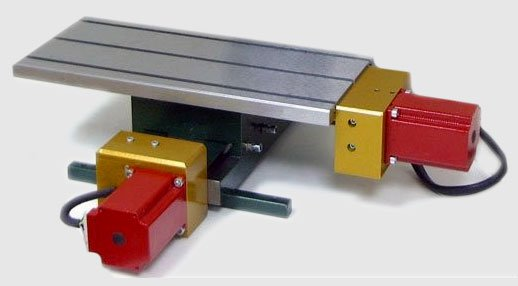
\includegraphics[scale=0.8]{ch-2/image10}
	}
	\caption{Координатный стол крестового типа.}\label{fig:cross}
\end{figure}

Можно выделить следующие недостатки крестовой конструкции координатных столов:

\begin{itemize}
	\item Данная кинематическая схема достаточно сложна в реализации, так как требует наличия жесткой связки линейных приводов, образующих рабочую крестовину.
	
	\item Увеличение массы перемещаемого объекта неизбежно ведет к необходимости увеличения мощности линейных приводов стола, что еще больше усложняет и удорожает конструкцию. Особенно это касается механизмов, где в дополнение к перемещению по координатам Х и Y, необходимо перемещение и по оси Z, то есть подъем или опускание крестовины относительно неподвижного рабочего органа. 
	
	\item Возможен прогиб осей по краям координатного стола.
\end{itemize}

Вторая разновидность координатных столов "--- портальная. Существует несколько компоновок портальных конструкций, отличающихся назначением и ограничениями областей применения. На рисунке~\cref{fig:coord-1} представлен координатный стол с неподвижным порталом, в~котором перемещение по оси Y осуществляется за счет продольного движения самого стола, а рабочий орган расположен на поперечной балке, которая может опускаться и подниматься, обеспечивая тем самым, движение по оси Z. Перемещение по оси X достигается за счет наличия дополнительного линейного привода, также расположенного на данной балке.

\begin{figure}[ht]
	\centerfloat{
		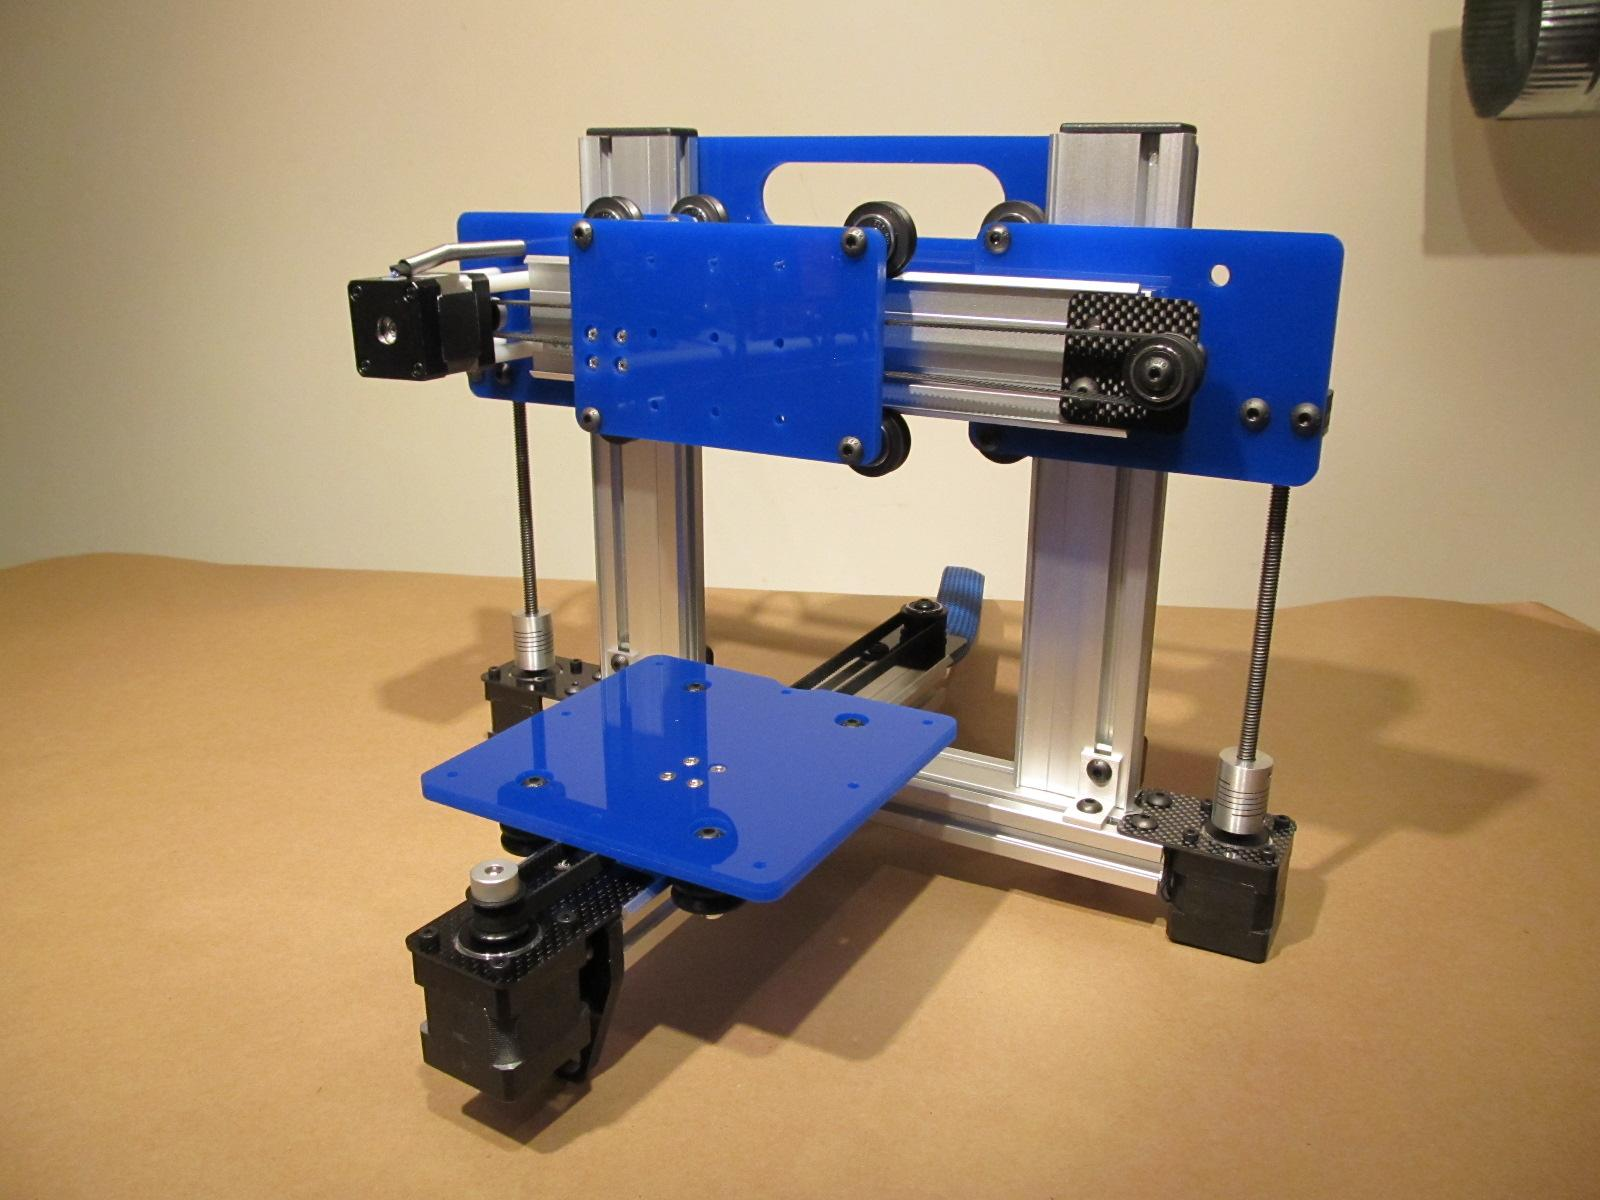
\includegraphics[scale=0.8]{ch-2/image11}
	}
	\caption{Координатный стол крестового типа.}\label{fig:coord-1}
\end{figure}

К достоинствам данной конструкции можно отнести:

\begin{itemize}
	\item высокую жесткость на изгиб;
	
	\item простоту изготовления.
\end{itemize}

Недостатками являются:

\begin{itemize}
	\item отсутствие возможности работы с объектами большой массы, так как подобные объекты должны крепиться и перемещаться по оси X, нагружая ее, что может привести к выходу из строя линейного привода или его изгиба.
	
	\item максимальные габаритные размеры объекта ограничены размерами портала.	
\end{itemize}

Также существуют конструкции, где неподвижный портал несет на себе балку, отвечающую только за перемещение рабочего органа по координате Z~(\cref{fig:coord-2}).

\begin{figure}[ht]
	\centerfloat{
		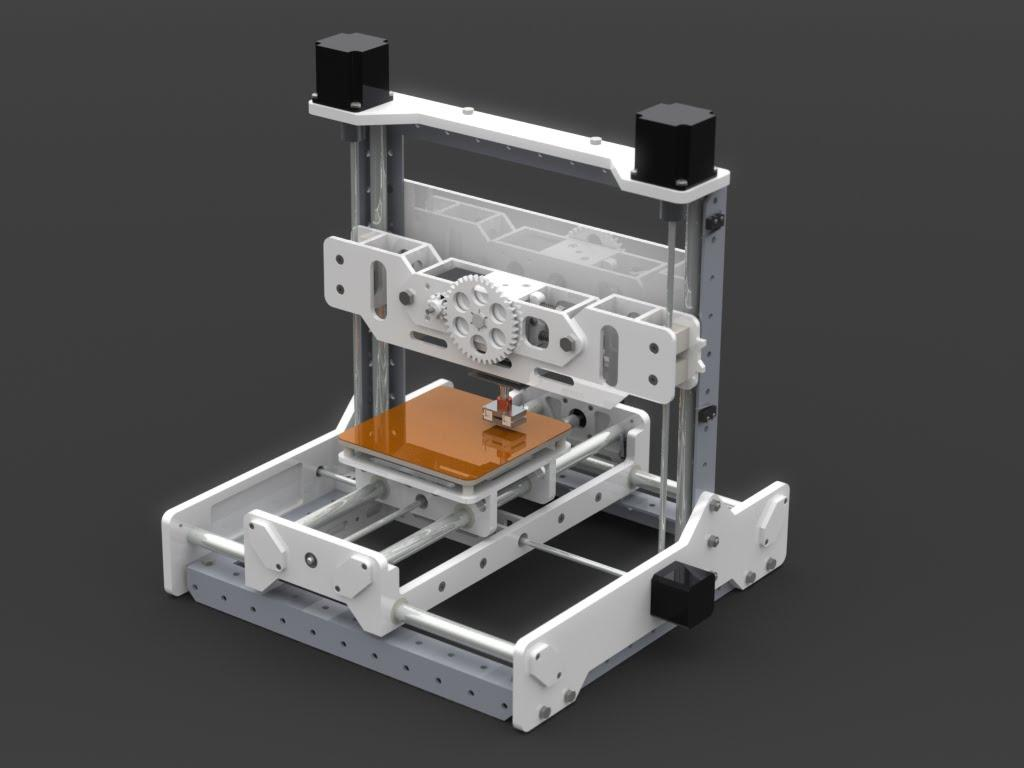
\includegraphics[scale=0.8]{ch-2/image12}
	}
	\caption{Второй вариант компоновки координатного стола с неподвижным порталом.}\label{fig:coord-2}
\end{figure}

Перемещение по координатам X и Y, как видно из рисунка, осуществляется за счет использования конструкции, похожей на крестовую, за исключением отсутствия единой точки крепления линейных приводов, что с одной стороны увеличивает жесткость конструкции и уменьшает прогиб по осям, а с другой "--- существенно сокращает рабочее поле стола.

Последний вариант конструкции с неподвижным порталом изображен на рисунке~\cref{fig:coord-3}. В данном механизме рабочий орган, размещенный на поперечной балке портала, обеспечивает перемещение по оси Y, в то время как рабочая поверхность может подниматься и опускаться (перемещение по оси Z), а также двигаться в поперечном по отношению к плоскости портала направлении (ось X). Очевидно, что подобная компоновка наиболее проста в реализации, но не является достаточно жесткой и не позволяет работать с объектами большой массы. Последнее определяет основную область применения данной кинематической схемы "--- изготовление недорогих трехмерных принтеров.

\begin{figure}[ht]
	\centerfloat{
		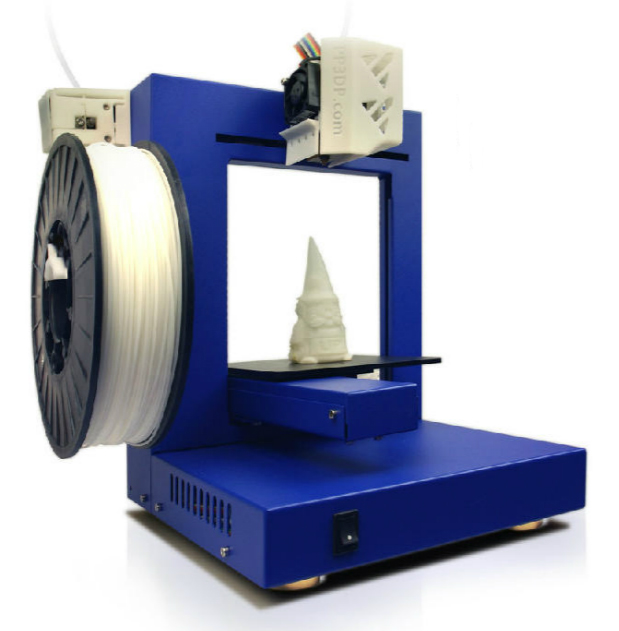
\includegraphics[scale=0.8]{ch-2/image13}
	}
	\caption{Третий вариант компоновки координатного стола с неподвижным порталом.}\label{fig:coord-3}
\end{figure}

Отдельно следует рассмотреть конструкцию координатного стола с подвижным порталом~(рисунок~\cref{fig:coord-4}).

\begin{figure}[ht]
	\centerfloat{
		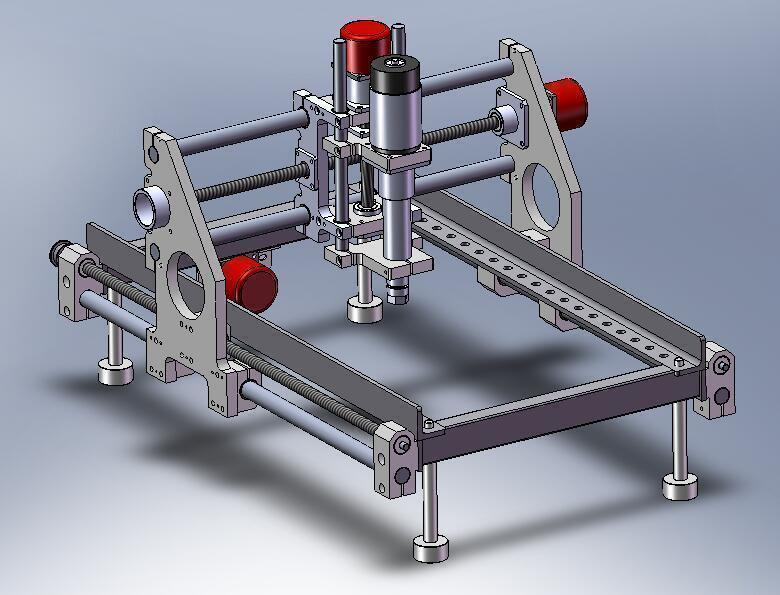
\includegraphics[scale=0.8]{ch-2/image14}
	}
	\caption{Конструкция координатного стола с подвижным порталом.}\label{fig:coord-4}
\end{figure}

Данная конструкция несколько сложнее предыдущих, так как сам портал и поперечная балка обеспечиваю перемещение рабочего органа по всем трем осям, рабочая поверхность стола при этом остается неподвижной. К очевидным достоинствам подобной кинематической схемы можно отнести:

\begin{itemize}
	\item достаточную простоту изготовления;
	
	\item универсальность и масштабируемость конструкции;
	
	\item ничем не ограниченный вес объекта;
	
	\item возможность встраивания в поточные линии (в качестве так называемого декартового робота);
	
	\item возможность работы с объектами, значительно превышающими габариты стола по оси Y, что находит применение при работе с листовыми материалами.
\end{itemize}

Основными недостатками конструкции являются:

\begin{itemize}
	\item необходимость использования очень жестких и прочных линейных приводов по оси Y, так как именно они будут испытывать максимальные нагрузки в процессе своей работы.
	
	\item зависимость жесткости и точности координатного стола от высоты портала, так как при увеличении размеров боковых стоек возможно увеличение их деформации и изгиба.
\end{itemize}

Анализ показал, что кинематическая схема координатного стола с подвижным порталом является наиболее распространенной при создании металлообрабатывающих и деревообрабатывающих станков координатно-фрезерного и координатно-сверлильного типов, механических, водоструйных, лазерных и плазменных резаков, различных граверов и режущих плоттеров и многих других видов оборудования с числовым программным управлением.

По совокупности достоинств и недостатков именно данная конструкция была принята в качестве наиболее близкого аналога кинематической схемы ШУТ. Однако для многих типов оборудования, разрабатываемых в соответствии с концепцией ADAPTEQ, третья координата вообще не требуется, для некоторых требуется, но с малым ходом и точностью, и лишь для самых сложных видов оборудования необходима полноценная высокоточная третья координата. В связи с этим в кинематической схеме ШУТ должна быть предусмотрена возможность регулировки портала по высоте, что позволит достичь максимальной точности и жесткости конструкции, сохранив при этом достаточно большие габариты рабочей области, а опциональную третью координату выполнить в качестве отдельного модуля, на котором будет крепиться рабочий орган~(рисунок~\cref{fig:coord-chassis}).

\begin{figure}[ht]
	\centerfloat{
		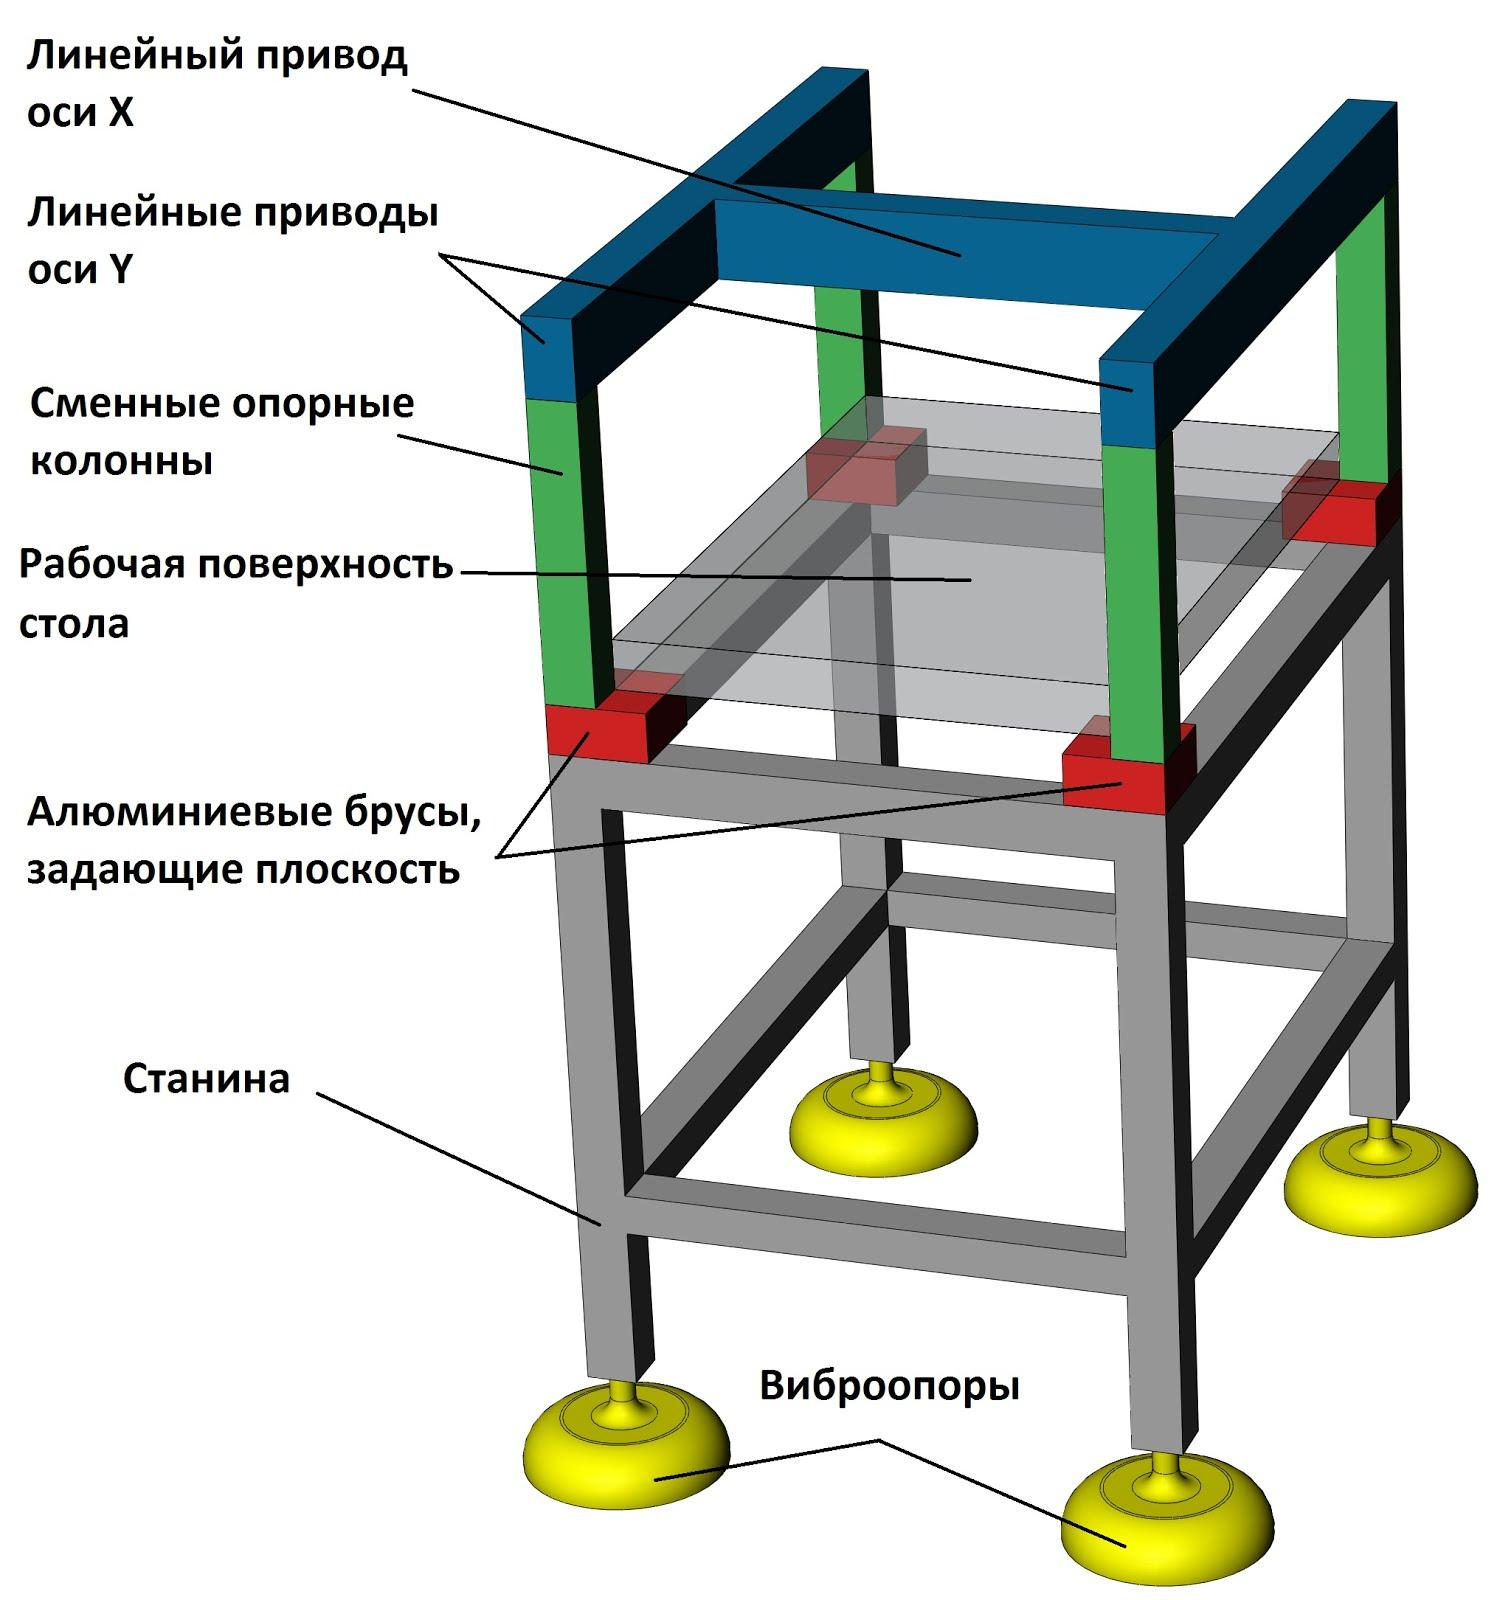
\includegraphics[scale=0.8]{ch-2/image15}
	}
	\caption{Общая компоновка ШУТ.}\label{fig:coord-chassis}
\end{figure}

Основание портала (станина) должна представлять собой сварную раму из стального проката (прямоугольные или квадратные трубы), по углам которой болтами необходимо закрепить четыре алюминиевых бруска, фрезеруемые совместно уже после крепления на раму. Бруски обеспечат плоскость, относительно которой можно базировать рабочую поверхность координатного стола и сменные опорные колонны, на которые будут опираться продольные и поперечные линейные приводы. Станина должна быть установлена на регулируемые по высоте виброопоры типов ОВ-31 и ОВ-70~(рисунок~\cref{fig:vibro}) в зависимости от общего веса конструкции.

\begin{figure}[ht]
	\centerfloat{
		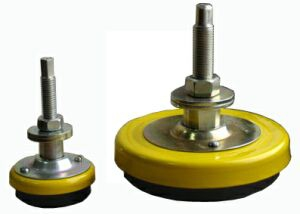
\includegraphics[scale=0.8]{ch-2/image16}
	}
	\caption{Виброопоры ОВ-31 (слева) и ОВ-70 (справа).}\label{fig:vibro}
\end{figure}

\textbf{2.4.2. Выбор линейных приводов ШУТ}

Линейный привод представляет собой конструкцию, являющуюся совокупностью механизмов, предназначенных для линейного перемещения исполнительных органов машин и приборов. В зависимости от вида преобразуемой энергии различают следующие виды линейных приводов:

\begin{itemize}
	\item линейные электроприводы;
	
	\item линейные гидроприводы;
	
	\item линейные пневмоприводы.
\end{itemize}

С точки зрения управления и реализации самыми простыми являются электроприводы, поэтому для реализации перемещения рабочего органа ШУТ будут применяться именно они.

Линейный привод состоит из трансмиссии, преобразующей вращательное движение в поступательное, и электродвигателя. Отдельно можно выделить линейный электродвигатель (или просто линейный двигатель).

\textit{Линейный двигатель}~(рисунок~\cref{fig:lindrive}) "--- это электродвигатель, один из элементов магнитной системы которого линейно развернут (он создает магнитное поле), а другой выполнен в виде подвижной каретки, перемещающейся в этом поле. На сегодняшний день существует несколько разновидностей линейных двигателей: линейные асинхронные электродвигатели, линейные синхронные электродвигатели, линейные электромагнитные двигатели, линейные магнитоэлектрические двигатели, линейные магнитострикционные двигатели, линейные пьезоэлектрические (электрострикционные) двигатели и~др.

\begin{figure}[ht]
	\centerfloat{
		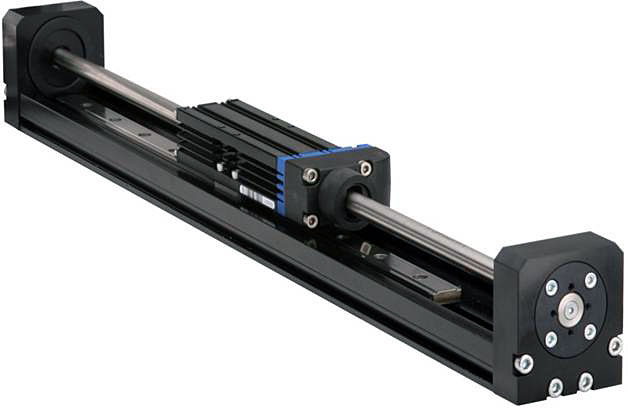
\includegraphics[scale=0.8]{ch-2/image17}
	}
	\caption{Цилиндрический линейный двигатель на постоянных магнитах.}\label{fig:lindrive}
\end{figure}

Основными достоинствами линейных двигателей являются:

\begin{itemize}
	\item \textit{Высокая скорость перемещения.} Максимальная скорость перемещения линейного двигателя ограничена только напряжением питания и производительностью управляющего контроллера (то есть его возможностью генерировать управляющие импульсы с максимально высокой частотой). Типичная скорость перемещения каретки линейного двигателя составляет 3 м/с при точности позиционирования 1 мкм и до 5 м/с при уменьшении точности. Очевидно, что для многих типов оборудования, проектируемого в рамках концепции ADAPTEQ, подобная скорость движения исполнительного органа будет избыточной.
	
	\item \textit{Высокая точность.} Точность, разрешающая способность и~повторяемость "--- те характеристики линейного двигателя, которые определяются обязательной для данного вида линейных приводов системой обратной связи по положению. Как правило, используются различные линейные системы контроля положения, выбор которых зависит в первую очередь от назначения и стоимости устройства, построенного на базе линейного двигателя.
	
	\item \textit{Очень высокое ускорение} (время разгона до номинальной скорости). Быстродействие линейного двигателя примерно в~сто раз больше, чем у аналогичных линейных электроприводов с трансмиссией, что позволяет использовать его в наиболее требовательных к этому параметру системах.
	
	\item \textit{Высокая жесткость.} В линейных двигателях отсутствует трансмиссия, поэтому жесткость, как характеристика сопротивления каретки линейного двигателя внешнему воздействию, может быть увеличена только за счет увеличения тока в обмотках якоря. Правда это увеличение не может быть бесконечно и зависит от сопротивления изоляции обмоток, системы охлаждения, необходимой точности позиционирования и т.\:д.
	
	\item \textit{Отсутствие люфта.} В линейных двигателях отсутствует свободный ход каретки по отношению к направляющей, что определяется отсутствием механической трансмиссии. Все ошибки позиционирования возникают только из-за несовершенства блока управления, система обратной связи по положению и качества изготовления деталей, генерирующих магнитное поле. Эти ошибки носят систематический характер и могут быть учтены в программе управления. 
\end{itemize}

Несмотря на все перечисленные достоинства, линейные двигатели не лишены и определенных недостатков. Перечислим те из них, которые по нашему мнению не позволяют использовать данный тип линейных приводов при создании ШУТ:

\begin{itemize}
	\item \textit{Стоимость}. Линейные двигатели стоят очень дорого. В~первую очередь это связано с необходимостью использования дорогих редкоземельных магнитов. Лучшие и~самые дорогие модели линейных двигателей создаются на базе цилиндрических направляющих (рельсов) с постоянными магнитами, расположенными по всей длине рельса. Очевидно, что стоимость такого привода растет пропорционально длине магнитных направляющих. Второй немаловажный фактор, влияющий на цену линейных двигателей "--- обязательная необходимость использования линейных датчиков, обеспечивающих обратную связь по положению. Данный тип датчиков является наиболее сложным и дорогим. Также стоит отметить, что линейные двигатели, как правило, требуют более сложного блока управления, построенного не на основе микроконтроллеров общего назначения, а на более дорогих цифровых процессорах сигнала (англ. \textit{Digital Signal Processor}, сокр. \textit{DSP}).
	
	\item \textit{Низкое тяговое усилие.} В сравнении с идентичными по массогабаритным характеристикам вращающимися двигателями, линейные двигатели развивают значительно более низкое тяговое усилие.
	
	\item \textit{Высокая рабочая температура.} В большинстве линейных двигателей якорь напрямую соединен с нагрузкой. КПД линейного двигателя может достигать 96\%, 4\% уходит в тепло, которому необходимо где-то рассеяться, поэтому в линейных двигателях высокой мощности обязательными являются системы принудительного воздушного или водяного охлаждения.
	
	\item \textit{Практически полное отсутствие трения.} В рабочем режиме якорь линейного двигателя находится в состоянии магнитной левитации, трение при этом минимально (только трение о~воздух). С одной стороны это достоинство линейных двигателей, а с другой "--- отсутствие трения означает и~отсутствие самоторможения. Например, представим вертикально расположенный линейный двигатель, якорь которого соединен с некоторой полезной нагрузкой и в данный момент находится в режиме удержания. Что произойдет в~случае потери питания? Если сила тяжести, действующая на якорь с закрепленной на нем полезной нагрузкой, окажется выше силы удержания постоянных магнитов в отсутствие магнитного поля, создаваемого катушками якоря, он просто упадет. Другой пример, якорь с полезной нагрузкой движется с максимальной скоростью (5 м/с), опять же происходит потеря питания. Единственное, что может остановить якорь "--- сила трения скольжения, возникающая между внутренней поверхностью якоря и доведенной поверхностью рельса. Очевидно, что при незначительной длине рельса ее будет недостаточно для быстрой остановки якоря, он ударится о концевую планку и может быть разрушен вместе с полезной нагрузкой.
	
	\item \textit{Высокое энергопотребление}. Анализ характеристик линейных двигателей показал, что при одинаковом тяговом усилии линейные двигатели потребляют больше электроэнергии, чем их вращающиеся аналоги.
	
	\item \textit{Не подлежат замене и модернизации.} Линейный двигатель является составной частью механизма, в котором он используется. Очевидно, что его крайне сложно заменить или модернизировать. Последнее явно противоречит принципу модульности, которому должно соответствовать оборудование, создаваемое в соответствии с концепцией ADAPTEQ.
\end{itemize}

Как уже было сказано ранее, \textit{линейные электроприводы с~трансмиссией} представляют собой совокупность механизма преобразующего вращательное движение двигателя в поступательное "--- цепи, зубчатого ремня, винтовой или шарико-винтовой пары (сокр. ШВП) и двигателя "--- шагового или серво. Рассмотрим эти элементы более подробно.

\textit{Цепная передача} осуществляет преобразование вращательно движения за счет использования специального многозвенного гибкого механизма, именуемого цепью. Связь цепи с валом электродвигателя осуществляется благодаря силам зацепления так называемой ведущей звездочки, также в конструкции должна быть предусмотрена вторая (ведомая звездочка), вращающаяся свободно и необходимая для создания замкнутого контура вращения и натяжения цепи. Количество зубьев в ведомой и ведущей звездочках должно совпадать, так как не требуется преобразование момента силы (передаточное отношение 1:1). При использовании цепной передачи каретка линейного привода перемещается по направляющим (рельсовым или цилиндрическим) и жестко связана с цепью. В случае большой нагрузки на линейный привод допускается использования многорядных цепей~(рисунок~\cref{fig:chain}).

\begin{figure}[ht]
	\centerfloat{
		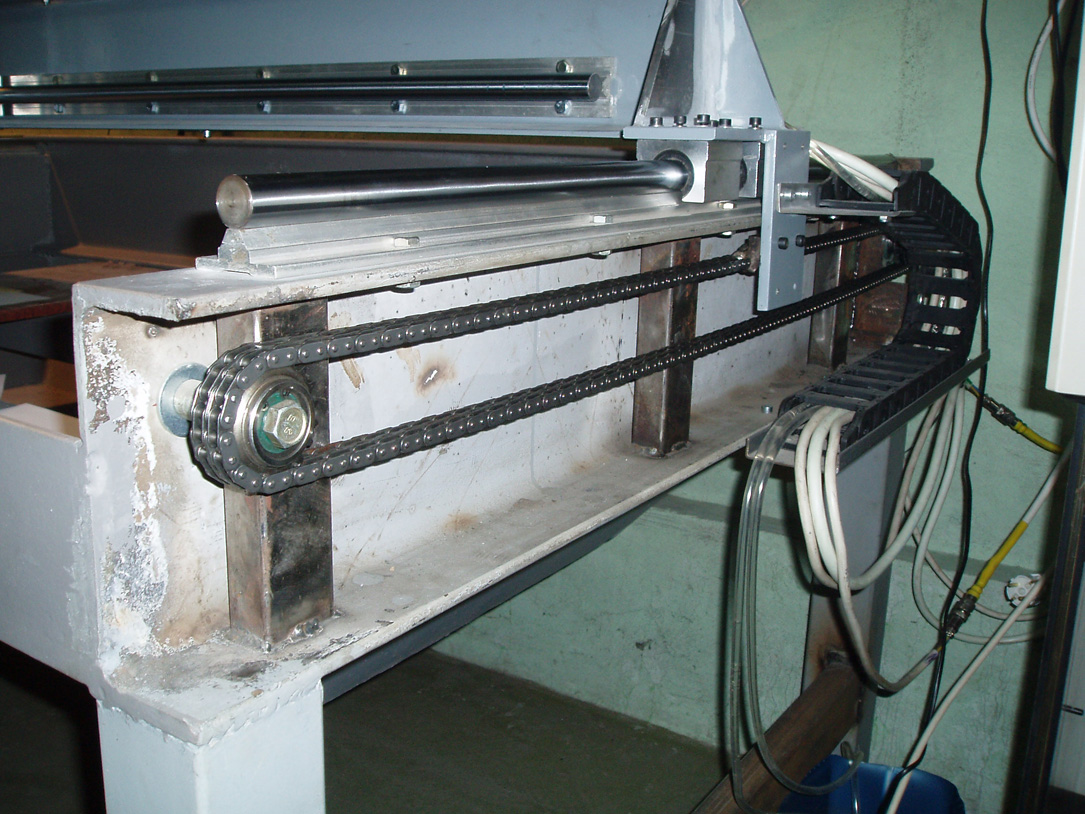
\includegraphics[scale=0.8]{ch-2/image18}
	}
	\caption{Пример многорядного цепного линейного привода.}\label{fig:chain}
\end{figure}

К достоинствам цепного линейного привода можно отнести:

\begin{itemize}
	\item Большая механическая прочность стальной цепи, позволяющая создавать высоконагруженные линейные приводы.
	
	\item Возможность создания достаточно габаритных линейных приводов.
	
	\item Достаточно высокий КПД (вплоть до 98\%).
	
	\item Отсутствие проскальзывания цепи.
	
	\item Незначительные нагрузки на ведущий и ведомый валы, так как не предполагается натяжение цепи.
\end{itemize}

К недостаткам следует отнести:

\begin{itemize}
	\item Цепная передача издает достаточно сильный шум и вибрацию.
	
	\item Качественные стальные цепи стоят дорого.
	
	\item Цепной механизм требует проектирования дополнительной системы постоянной смазки.
	
	\item Скорость движения цепи, особенно на малых скоростях, непостоянна, что не позволяет использовать подобный тип линейных приводов в прецизионном оборудовании.
	
	\item Износ механических сопряжений звеньев приводит к постепенному ослаблению цепи (цепь изначально не перетянута), поэтому в конструкции линейного привода должна быть предусмотрена хотя бы одна <<паразитная>> звездочка, связанная с жесткой пружиной, обеспечивающей гашения вибрации и натяжение цепи.
	
	\item При обрыве цепи может быть поврежден остальной механизм линейного привода.
\end{itemize}

Логическим развитием цепных линейных приводов являются приводы на зубчатых ремнях~(рисунок~\cref{fig:belt}). Данный тип передачи обладает всеми достоинствами цепной передачи, но лишен многих ее недостатков (плавность работы, бесшумность, более низкая стоимость, отсутствие необходимости в смазке и т.~д.). 

\begin{figure}[ht]
	\centerfloat{
		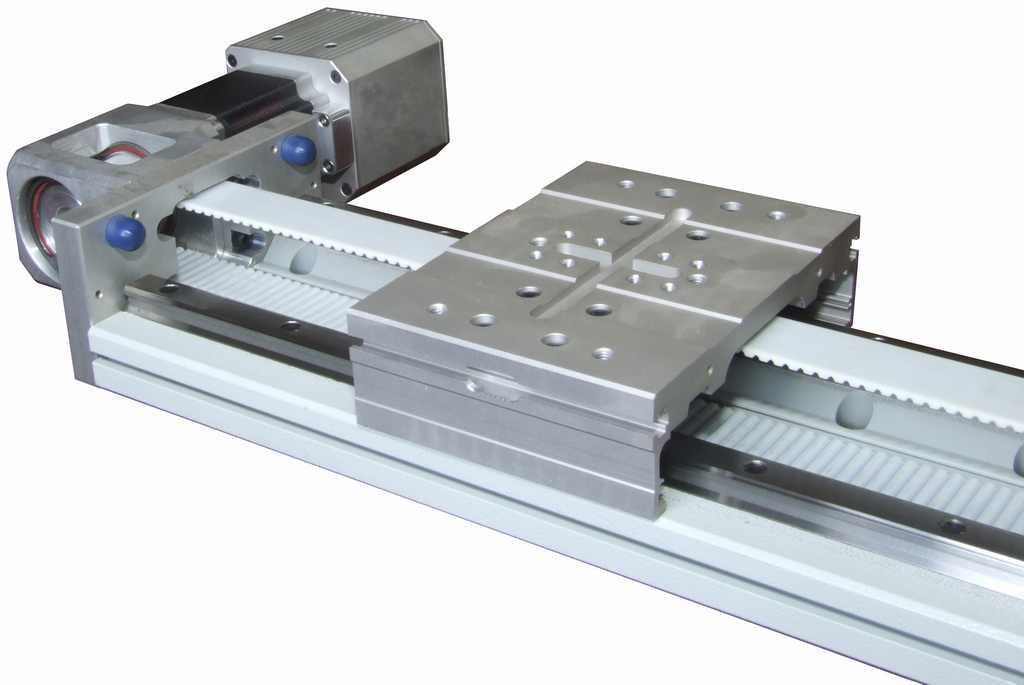
\includegraphics[scale=0.8]{ch-2/image19}
	}
	\caption{Линейный привод на основе зубчатого ремня.}\label{fig:belt}
\end{figure}

Линейные приводы на основе зубчатых ремней нашли широкое применение в современном высокоточном оборудовании, однако было принято решение не использовать ее при проектировании линейных приводов ШУТ. Данное решение обосновано необходимостью создания не просто надежного и универсального механизма перемещения потального типа, но и желанием добиться избыточности по некоторым параметрам, например, получить привод с максимально возможной нагрузочной способностью без увеличения габаритов и сложности конструкции. По этой причине предпочтение было отдано винтовой передаче. При этом зубчатый ремень тоже будет использован, но только как вспомогательный механизм (о чем будет сказано далее в этом разделе).

Перейдем к рассмотрению винтовых передач, а точнее шариково-винтовых пар~(рисунок~\cref{fig:ballscrew}), так как именно этот тип является наиболее распространенным на сегодняшний день\footnote{Передачи скольжения не рассматривались в силу их морального устаревания.}.

Шариково-винтовая пара является разновидностью передачи качения, в которой промежуточными телами являются закаленные шарики. Конструктивно шариково-винтовая пара состоит из винта и гайки с~канавками специального профиля. Шарики движутся по замкнутой траектории, проходящей через канавки винта и витки гайки через перепускные каналы (возвратные трубки), находящиеся в специальных вкладышах, расположенных в окне гайки.

Парные витки гайки продольно смещены по отношению к канавкам винта в двух направлениях, что обеспечивает преднатяг механизма и~компенсацию возможного люфта~(рисунок~\cref{fig:ballscrew-1}). Также в конструкции шариково-винтовой пары предусмотрены лубрикаторы, обеспечивающие постоянную смазку механизма густой смазкой, и грязесъемные кольца.

\begin{figure}[ht]
	\centerfloat{
		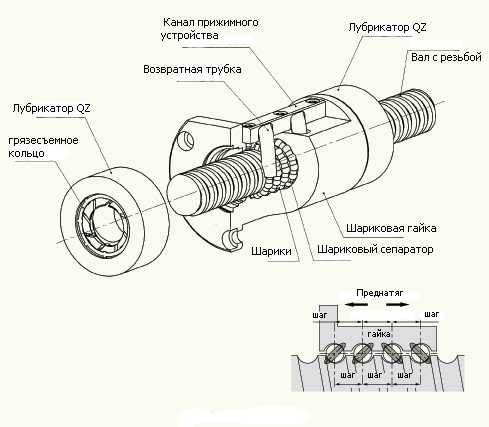
\includegraphics[scale=0.8]{ch-2/image20}
	}
	\caption{Конструкция шарико-винтовой пары.}\label{fig:ballscrew}
\end{figure}

\begin{figure}[ht]
	\centerfloat{
		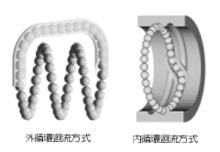
\includegraphics[scale=0.8]{ch-2/image21}
	}
	\caption{Схема движения тел качения в шариково-винтовой паре.}\label{fig:ballscrew-1}
\end{figure}

Основные достоинства шарико-винтовой пары:

\begin{itemize}
	\item Высокий КПД, определяющийся малыми потерями на трение.
	
	\item Большая нагрузочная способность при достаточно малых габаритах.
	
	\item Высокая точность перемещения, обусловленная практически полным отсутствием люфта.
	
	\item Самоторможение механизма при выходе из строя двигателя привода.
	
	\item Высокое быстродействие, определяемое значительной скоростью вращения винта.
	
	\item Плавный ход и бесшумность.
\end{itemize}

Из выявленных недостатков можно выделить следующие:

\begin{itemize}
	\item Сложность конструкции гайки.
	
	\item Достаточно высокая в сравнении с передачей на зубчатом ремне цена.
\end{itemize}

Тем не менее, именно конструкция линейного привода на основе шариково-винтовой пары признана наиболее оптимальной и~удовлетворяющей основным требованиям к ШУТ. 

Последний этап проектирования линейного привода "--- выбор двигателя. Выбор делался между двумя типами вращающихся двигателей: шаговых и серводвигателей. Данные типы имеют принципиальные конструктивные отличия. Шаговый двигатель является синхронным бесколлекторным двигателем с несколькими парными обмотками, расположенными в статоре~(рисунок~\cref{fig:stepper}). Подача тока на одну из обмоток приводит к изменению положения ротора (его фиксацию по отношению к~одному из полюсов многополюсного постоянного магнита ротора). Циклическая активация (переключение) обмоток вызывает дискретные угловые перемещения ротора, именуемые шагами.

\begin{figure}[ht]
	\centerfloat{
		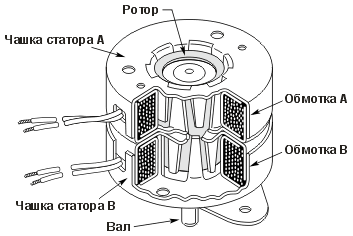
\includegraphics[scale=0.8]{ch-2/image22}
	}
	\caption{Конструкция шагового двигателя.}\label{fig:stepper}
\end{figure}

Серводвигатель~(рисунок~\cref{fig:servo}) представляет собой обычный электрический двигатель (как правило, постоянного тока, снабженный понижающим зубчатым редуктором или без него, в зависимости от требований к создаваемому моменту на валу двигателя) с обязательной схемой управления с отрицательной обратной связью по положению вала. Для обеспечения обратной связи используются датчики угла поворота различных конструкций, начиная с простейших потенциометров и~заканчивая прецизионными оптическими или магнитными энкодерами.

Перейдем к рассмотрению достоинств и недостатков двигателей обоих типов. Основными достоинствами \textit{серводвигателей} являются:

\begin{itemize}
	\item В случае использования механического редуктора серводвигатель может создавать достаточно большое для своих габаритов и массы усилие на валу.
	
	\item Точность позиционирования серводвигателя определяется типом используемого датчика углового положения и может быть достаточно высокой.
	
	\item Высокий КПД, достигающий 90\% при малых нагрузках.
	
	\item Низкая инертность и способность к очень быстрому ускорению даже при высокой нагрузке.	
\end{itemize}

\begin{figure}[ht]
	\centerfloat{
		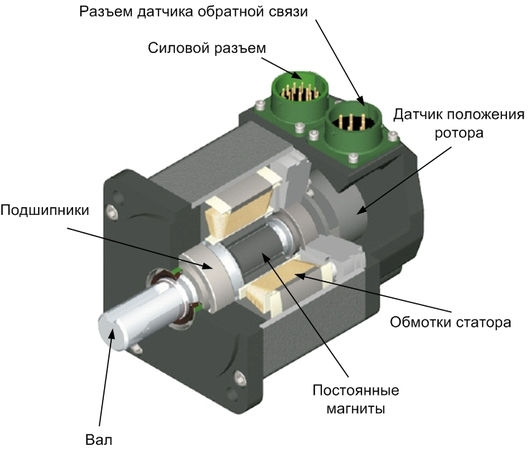
\includegraphics[scale=0.8]{ch-2/image23}
	}
	\caption{Конструкция безредукторного серводвигателя, созданного на основе трехфазного бесколлекторного двигателя постоянного тока.}\label{fig:servo}
\end{figure}

\begin{itemize}
	\item Низкая рабочая температура, так как ток потребляется пропорционально нагрузке.
	
	\item Пиковая мощность и крутящий момент могут быть в несколько раз больше номинальных, что позволяет использовать серводвигатели в жестких условиях эксплуатации (естественно, если будет создана система экстренного охлаждения).
	
	\item Серводвигатели работают плавно и практически бесшумно даже на больших скоростях.
	
	\item Серводвигатели не подвержены влиянию резонанса и~вибрации на всем диапазоне рабочих частот.
\end{itemize}

К недостаткам серводвигателей можно отнести:

\begin{itemize}
	\item Мощные серводвигатели требуют создания воздушной системы охлаждения, вентиляционные каналы которой могут засоряться в процессе работы.
	
	\item Максимальный момент серводвигатели отдают на очень высоких оборотах, поэтому как правила должны изготавливаться в сборе с редуктором.
	
	\item Требуют достаточно мощных и защищенных от кратковременных перегрузок источников питания.
	
	\item В случае заклинивания механизма или длительной перегрузке серводвигатель можно быстро перегореть. Единственный способ борьбы с этим явлением использование дополнительных датчиков нагрузки и специальной программы управления не допускающей длительных перегрузок.
	
	\item Сложный алгоритм управления, который требует использования дорогостоящих контроллеров, энкодеров и~предварительной калибровки и настройки, так как основной алгоритм управления данным типом двигателя предполагает создания пропорционально-интегрально-дифференциального регулятора.
	
	\item Более высокая по сравнению с шаговыми двигателями стоимость, обусловленная необходимостью использования дорогостоящих редукторов, энкодеров и схем регулирования и~управления.
\end{itemize}

Достоинствами \textit{шаговых двигателей} являются:

\begin{itemize}
	\item Высокая точность и стабильность шага, не зависящая от приложенной нагрузки.
	
	\item Не требует наличия обратных связей по положению, так как имеет фиксированный угол поворота.
	
	\item Шаговые двигатели являются очень распространенными и~производятся повсеместно, что определяет их невысокую стоимость. В случае поломки его можно просто заменить.
	
	\item Более долгий по сравнению с серводвигателями срок эксплуатации.
	
	\item Более простая система управления. Существует огромное количество готовых интегральных драйверов, сочетающих в~себе силовую часть и блок управления, которому нужен только тактовый сигнал от микроконтроллера. В простейшем случае можно обойтись только силовой частью, а~последовательность шагов генерировать с помощью микроконтроллера.
	
	\item В случае превышения максимальной нагрузки двигатель не сгорает, так как работа в режиме удержания является для него штатным режимом.
	
	\item Обеспечивает достаточный крутящий момент даже на низких оборотах, что не требует применения редукторов.
	
	\item Отличная повторяемость, как правило, в штатном режиме шаговый двигатель не должен пропускать шаги.	
\end{itemize}

Недостатки шаговых двигателей следующие:

\begin{itemize}
	\item Высокое энергопотребление, не зависящее от нагрузки.
	
	\item Пропорциональное снижение крутящего момента с~повышением оборотов.
	
	\item Низкая точность, обусловленная тем, что шаг задается полюсами постоянного магнита ротора, количество, которых по понятным причинам не может быть очень большим. Стандартное количество шагов для большинства шаговых двигателей 200 или 400. Низкая точно частично может быть скомпенсирована использованием микрошагового режима, который реализуется в блоке управления и позволяет ротору находиться в промежуточном положении между полюсами, а~также возможностью применения внешних съемных редукторов, которые лишь немного увеличивают габариты шагового двигателя.
	
	\item Возможно появление резонанса, что опять же может быть скомпенсировано применением микрошага.
	
	\item Полное отсутствие контроля положения вала.
	
	\item Даже в штатном режиме шаговый двигатель ощутимо нагревается, однако конструкция шагового двигателя позволяет эффективно рассеивать это тепло, система принудительно охлаждения, как правило, не требуется.
	
	\item Под нагрузкой не может начать движение сразу на высокой скорости. Требуется реализация плавного разгона и~торможения.
	
	\item Не может мгновенно восстанавливаться после перегрузки.
	
	\item Значительно шумит на средних и высоких скоростях, что также частично компенсируется использованием микрошага.
	
	\item Для своих габаритов и массы имеет недостаточную по сравнению с серводвигателями мощность.
\end{itemize}

Анализ показал, что оба типа двигателей удовлетворяют всем требованиям, предъявляемым к ШУТ. Поэтому было найдено следующие компромиссное решение: основные линейные приводы координатного стола (обеспечивающие перемещение по координатам X и Y), а также линейный привод опциональной координаты Z приводятся в движение шаговыми двигателями без редукторов с количеством шагов, равном 400 (максимальное количество шагов для двигателей данного типа).

При этом на осях предусматривается крепление для вращающихся оптических инкрементальных энкодеров, контролирующих положение шариково-винтовых пар и не допускающих пропуск шагов. Разрешающая способность энкодеров должна быть в несколько раз выше количества шагов.

Для обеспечения плавности хода и снижения явления вибрации предполагается применение недорого интегрального драйвера с~возможностью генерации микрошага (16--32 микрошага). Повышение точности позиционирования за счет использования микрошага не предполагается, программа управления работает только с целыми шагами, опираясь на показания датчиков положения. Компенсация погрешности позиционирования задается реализацией простейшего пропорционального регулятора.

\textbf{2.4.3. Итоговая схема компоновки координатного стола ШУТ}

На рисунке~\cref{fig:scheme} представлена итоговая Электрокинематическая схема координатного стола ШУТ. Перемещение рабочего органа по оси Y осуществляется за счет поперечной опорной балки, перемещающейся по направляющим 10. Направляющие выполнены из закаленного круглого прутка с опорой, поперечная балка опирается на ползуны с разрезными линейными подшипниками 5. Конструкция направляющих представлена на рисунке~\cref{fig:bearing}, также для увеличения жесткости конструкции предлагается разместить направляющие на основании, выполненном из стальной трубы прямоугольного профиля.

Для предотвращения заклинивания поперечной балки при движении по направляющим применена классическая схема, с размещение с одной стороны балки двух разнесенных по отношению друг к другу подшипников, а с другой "--- одного. Ползуны соединены с гайкой шариково-винтовой пары 7, опирающейся с двух сторон на радиальные подшипники 4 и 6. Шариково-винтовая пара располагается непосредственно над опорной направляющей и является полностью разгруженной, то есть не испытывает никаких радиальных нагрузок. На поперечной балке также размещена цилиндрическая направляющая и шариково-винтовая пара оси X.

\begin{figure}[ht]
	\centerfloat{
		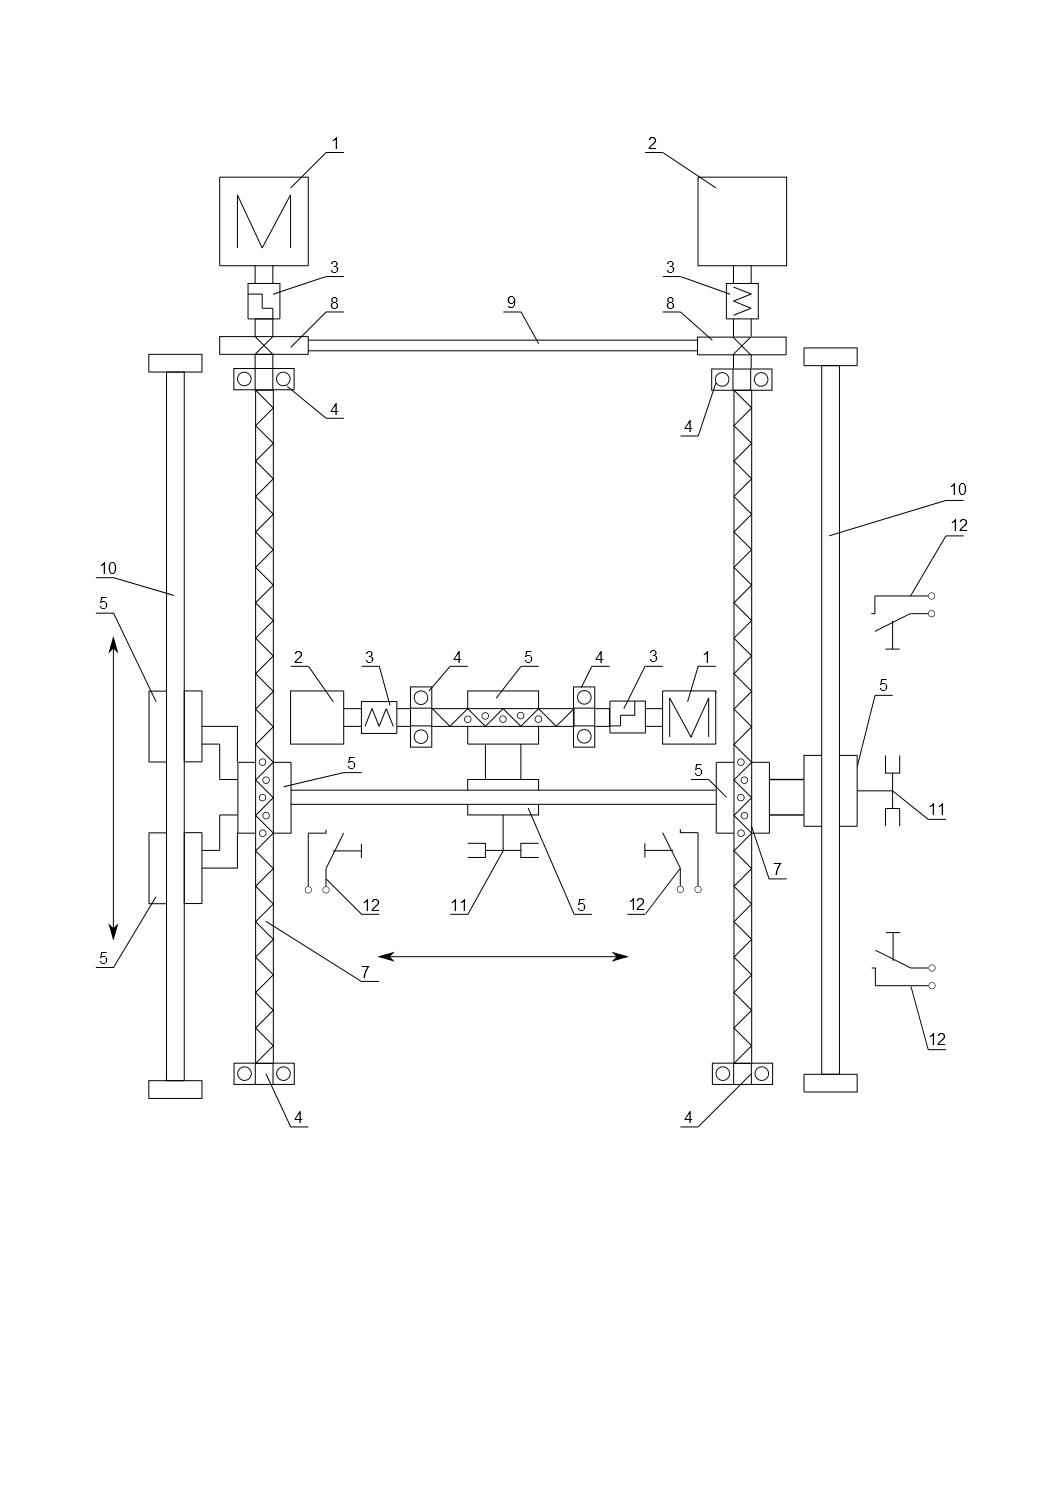
\includegraphics[scale=0.8]{ch-2/image24}
	}
	\caption{Электрокинематическая схема координатного стола ШУТ.}\label{fig:scheme}
\end{figure}

\begin{figure}[ht]
	\centerfloat{
		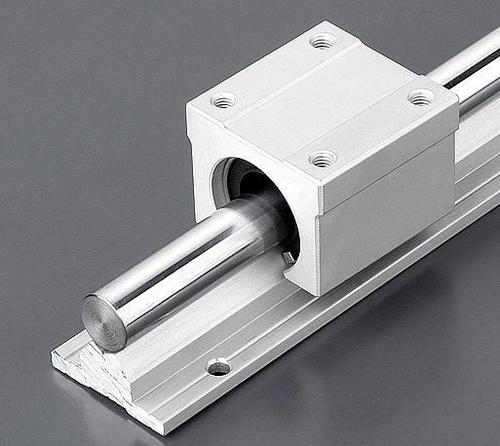
\includegraphics[scale=0.8]{ch-2/image25}
	}
	\caption{Разрезной линейный подшипник и цилиндрическая направляющая с опорой.}\label{fig:bearing}
\end{figure}

Ползун оси X соединен с плоскостью универсального крепления рабочего органа или сменного модуля.

Вращение шарико-винтовых пар осуществляется с помощью шагового двигателя 1 форм-фактора NEMA23 с квадратным фланцем со стороной 57 мм (экспериментальный образец будет создан на основе китайских двигателей FL57STH76-3005MA с разрешением 400 шагов на оборот). Сопряжение двигателя с шарико-винтовой пары достигается за счет кулачковой муфты 3. Синхронизация валов обеспечивается зубчатым ремнем 9 и зубчатыми шкивами 8, также предусмотрена система натяжения ремня, представляющая собой свободно вращающийся шкив и пружину сжатия.

Обратная связь по положение достигается использованием вращающихся инкрементальных энкодеров 2 (предполагается использование отечественных датчиков, например, ЛИР-158).

Энкодеры сопрягаются с шариково-винтовой парой путем использования сильфонных муфт. Для оси Y датчик крепится не на основной шариково-винтовой паре, а на вспомогательной, синхронизированной через зубчатый ремень. Таким образом, отсутствует необходимость использования отдельного датчика обрыва ремня. 

Каждая ось ШУТ снабжена двумя механическими концевыми выключателями 12. Функция концевых выключателей "--- экстренный останов ползуна при достижении края направляющей для предотвращения поломок от их соударения. Концевые выключатели подключены в обход основной схемы управления и не зависят от основного управляющего контроллера. Система экстренной остановки будет работать даже в случае зависания или выхода из строя основного микроконтроллера управления. Последнее достигается за счет использования простой логической схемы, которая при замыкании любого из двух концевых выключателей оси переводит шаговый двигатель в режим удержания (питание подается на обе фазы одновременно, благодаря чему происходит магнитное торможение двигателя). В конструкции также предусмотрены концевые противоударные элементы, выполненные в виде резиновых, пружинных или тросовых гасителей.

На обоих ползунах размещены щелевые оптически датчики 11, необходимые для самокалибрования ШУТ. Предполагается, что каждый раз при включении установки ползуны обеих осей будут на минимальной скорости перемещаться в одном направлении до срабатывания первого оптического датчика, а затем в противоположном до второго. При этом энкодер зафиксирует, сколько шагов можно будет сделать по каждой из осей, зафиксировав тем самым нулевую и максимальную координату каждой из осей. Данный подход позволяет компенсировать любые деформации механизма, возникающие, например, из-за перепада температуры.

\textbf{2.4.4. Изготовление ШУТ}

По своей конструкции ШУТ является достаточно простым механизмом. Предполагается, что прототип ШУТ может быть изготовлен только с применением недорогого универсального оборудования. Как уже было отмечено в разд. 2.2 основная область применения ШУТ, являющейся основой любого оборудования, удовлетворяющего требованиям концепции ADAPTEQ, это малые инновационные предприятия. Понятие МИП включает в себя инжиниринговые центры, малые производства и промышленные лаборатории (сокр. \textit{промлаб}). Рассмотрим процесс изготовления ШУТ и необходимое для этого оборудование на примере промлаба.

Процесс изготовления ШУТ начинается с изготовления опорной рамы или станины. Станина представляет собой сварную конструкцию из стальных труб квадратного или прямоугольного сечения. Вначале необходимо разметить заготовки, в качестве которых выступают хлысты проката, для этого в арсенале промлаба должен быть различный измерительный инструмент: стальная линейка, штангенциркуль, угольник, а также твердосплавная чертилка для разметки труб.

Трубы отрезаются не в размер, а с запасом \SIrange{5}{10}{\milli\metre}. Рез осуществляется с помощью отрезного круга или ручной углошлифовальной машинки, в просторечии, именуемой <<болгаркой>>.

После отрезания концы заготовок должны быть доработаны на фрезерном станке, после чего края заготовок должны быть зачищены от возникших в процессе обработки заусенцев (для этого используются различные слесарные инструменты: напильники, тиски и~т.\:д.).

После слесарной обработки заготовки размещаются на верстаке и~закрепляются с помощью струбцин для сварки. Сварка осуществляется с~помощью ручного или полуавтоматического сварочного аппарата. После сварки при необходимости производится зачистка сварных швов и~покраска рамы из пульверизатора, подключенного к компрессору.

Следующий этап "--- изготовление брусов, задающих плоскость. Брусы отрезаются от заготовки, после чего обрабатываются на фрезерном станке и крепятся на раме с помощью болтовых соединений. Для этого необходимо разметить отверстия на раме и брусах с помощью керна, а затем просверлить отверстия на сверлильном станке или ручной дрелью, затем доработать их с помощью зенкера и развертки и зачистить заусенцы. После того, как все четыре бруса будут размещены по углам рамы, необходимо обработать их совместно на фрезерном станке. Рабочая поверхность стола и опорные колонны также изготавливаются на фрезерном станке.

Элементы линейных приводов изготавливаются на фрезерном и токарном станках, при этом могут понадобиться дополнительные измерительные инструменты, например, нутромер, микрометр, поверочная плита и~т.\:д. Для окончательной сборки ШУТ необходимы только ручные инструменты: отвертки, ключи и~др.

\textbf{2.5. Универсальный блок управления и программное обеспечение}

\textbf{2.5.1. Универсальный блок управления}

Универсальный блок управления является центральным компонентом \foreignlanguage{english}{ADAPTEQ}, так как позволяет связать аппаратную часть создаваемого на базе этой концепции оборудования (занимается получением данных от датчиков ШУТ и рабочих органов, генерирует управляющие сигналы приводов) и программную часть (связывает оборудование с ПК и позволяет осуществлять двухсторонний обмен данными с \foreignlanguage{english}{TAPS}). Универсальный блок управления будет состоять из следующих модулей:

\begin{itemize}
	\item Модуль питания.
	
	\item Процессорный модуль.
	
	\item Модуль сопряжения с ПК.
	
	\item Модуль сопряжения с датчиками.
	
	\item Модули управления приводами.
	
	\item Модуль индикации и взаимодействия с оператором.
\end{itemize}

Предполагается, что все модули будут снабжены собственным микроконтроллером, обеспечивающим их взаимодействие по протоколу \foreignlanguage{english}{SPI}\footnote{сокр.~от~англ. англ. \textit{Serial Peripheral Interface, SPI bus} "--- последовательный периферийный интерфейс, шина SPI.} Данный протокол позволит всем модулям соединяться между собой и обмениваться необходимой информацией в синхронном последовательном режиме. То есть универсальный блок управления будет представлять собой сеть микроконтроллеров, обеспечивающих различные функции.

В качестве \textit{модуля питания} предполагается взять стандартный промышленный блок питания, работающий на напряжении~\SI{48}{\volt} постоянного тока и обеспечивающий мощность порядка~\SIrange{400}{500}{\watt}.

Для получения различных напряжений, необходимых, например, для питания микроконтроллера, датчиков, двигателей, энкодеров и~др. предполагается создание сменных плат питания, построенных на базе современных импульсных стабилизаторов напряжения с высоким КПД таких, как \foreignlanguage{english}{LM}2940, \foreignlanguage{english}{LT}1185, \foreignlanguage{english}{LT}1528 и~др. Подобные регуляторы могут обеспечивать ток до~\SI{3}{\ampere} (возможно запараллеливание для достижения больших значений тока), требуют минимальной обвязки и очень дешевы, выходное напряжение в них задается подстроечным резистором, который после настройки каждой платы должен быть опломбирован.

\textit{Процессорный модуль} будет выполнять функции по управлению ШУТ, получению и обработке данных, полученных от других модулей, а также вспомогательные функции, например, индикация и взаимодействие с оператором.

Наиболее важная функция программного обеспечения универсального блока управления "--- получение и обработка \foreignlanguage{english}{G}-кодов, полученных от ПК (интеграция с \foreignlanguage{english}{TAPS}).

Модуль будет построен на базе тридцатидвухбитного процессора семейства \foreignlanguage{english}{ARM}. Выбор обусловлен имеющимся положительным опытом работы с микроконтроллерами этого семейства архитектур, в частности, использовались контроллеры \foreignlanguage{english}{STMicroelectronics}, \foreignlanguage{english}{Texas Instruments}, \foreignlanguage{english}{NXP} и~др. Для данного проекта предполагается использование отечественных микроконтроллеров, производимых ЗАО~<<ПКК Миландр>>.

\textit{Модуль сопряжения с ПК} необходим для взаимодействия с исполнительными устройствами и датчиками оборудования, построенного на базе концепции \foreignlanguage{english}{ADAPTEQ}. Предполагается, что обмен данными между универсальным блоком управления будет осуществляться через стек протоколов \foreignlanguage{english}{TCP/IP}\footnote{сокр.~от~англ. \textit{Transmission Control Protocol/Internet Protocol} "--- протокол передачи данных/интернет-протокол.}, на прикладном уровне будет использован протокол \foreignlanguage{english}{HTTPS}\footnote{сокр.~от~англ. \textit{HyperText Transfer Protocol Secure} "--- защищенный протокол передачи гипертекста.} с самоподписанным сертификатом; на канальном "--- возможно использование протоколов \foreignlanguage{english}{Ethernet} (для проводного соединения) и IEEE 802.11 Wireless Ethernet (для беспроводного). Подобная реализация позволит легко интегрировать оборудование, построенное в соответствие с концепцией \foreignlanguage{english}{ADAPTEQ} в существующую локальную сеть (включая возможность доступа через Интернет), а также позволит работать с ним без установки каких-либо драйверов или другого вспомогательного программного обеспечения. Программная реализация данного взаимодействия будет рассмотрена в следующем разделе.

\textit{Модуль сопряжения с датчиками} будет обрабатывать информацию, полученную от датчиков. Предполагается, что большинство современных датчиков являются либо аналоговыми, либо цифровыми и работают по одному из протоколов взаимодействия: \foreignlanguage{english}{SPI}, \foreignlanguage{english}{I}2\foreignlanguage{english}{C}, 1-\foreignlanguage{english}{Wire}, \foreignlanguage{english}{CAN} (сокр.~от~англ. \textit{Controller Area Network} "--- сеть контроллеров).

В случае использования аналоговых датчиков, сигнал должен быть усилен с~помощью операционного усилителя и оцифрован посредством аналогово-цифрового преобразователя (сокр. \textit{АЦП}). Оба этих компонента имеют возможность программного управления, то есть необходимость усиления сигнала, разрядность АЦП и другие параметры могут быть заданы отдельно для каждого аналогового датчика.

Если же сигнал цифровой, необходимо согласование протокола, по которому работает датчик и внутреннего протокола универсального блока управления "--- \foreignlanguage{english}{SPI}. Согласование осуществляется программно на этапе первичной настройки универсального блока управления под конкретный тип оборудования.

Дополнительно модуль сопряжения с датчиками будет включать в~себя подмодуль преобразования логических уровней, так как возможно несовпадение напряжения питания какого-либо датчика с основным логическим напряжением универсального блока управления (для процессоров семейства \foreignlanguage{english}{ARM}, как правило, логические уровни задаются напряжением от 0 до 3,3~В).

\textit{Модули управления приводами} являются силовыми и позволяют управлять шаговыми двигателями и прочими электродвигателями, используемыми в оборудовании, создаваемом на базе концепции \foreignlanguage{english}{ADAPTEQ}. Например, для управления шаговыми двигателями, модули могут быть построены на базе популярных интегральных драйверов шаговых двигателей, например, \foreignlanguage{english}{L}297+\foreignlanguage{english}{L}298, \foreignlanguage{english}{DRV}8825 или \foreignlanguage{english}{TB}6600. В~зависимости от задач, решаемых конкретным типом оборудования, возможно использование и более сложные и дорогие схемы управления двигателями, при этом универсальность достигается единым протоколом взаимодействия с процессорным модулем. Предполагается, что процессорный модуль при необходимости будет взаимодействовать с 8 модулями управления приводами.

\textit{Модуль индикации и взаимодействия с оператором} позволяет отображать важную информацию о текущем состоянии оборудования с~помощью различных типов индикаторов (сегментных, жидкокристаллических и~др.), а также взаимодействовать с оператором без подключения к ПК.

Данный модуль необходим для первичной настройки оборудования (например, присвоения внутреннего адреса в локальной сети, к которой оно будет подключено или параметров беспроводной точки доступа), восстановления после сбоев и прочих операций, которые невозможно или нецелесообразно производить через основной интерфейс управления. Данный модуль является опциональным и все его функции должны быть продублированы в основном интерфейсе взаимодействия с оборудованием, реализуемым на ПК.

\begin{figure}[ht]
	\centerfloat{
		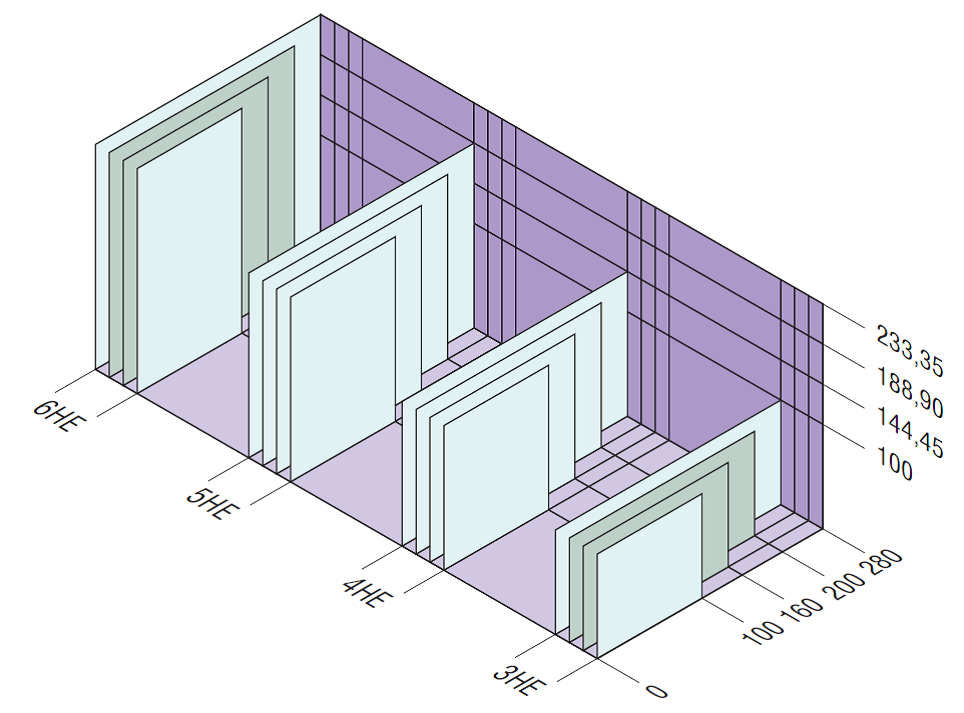
\includegraphics[scale=0.8]{ch-2/image26}
	}
	\caption{стандартные типоразмеры печатных плат модулей универсального блока управления.}\label{fig:euromech}
\end{figure}

Конструктивно все модули должны быть выполнены по стандарту МЭК 60297 (известному как <<Евромеханика>>), то есть с возможностью размещения в стандартных корзинах девятнадцатидюймовых телекоммуникационных стоек. Типоразмеры печатных плат, удовлетворяющих данному стандарту, представлены на рисунке~\cref{fig:euromech} (\foreignlanguage{english}{HE} "--- единица, в которой задаётся ширина конструкции, равна 5,08 мм (0,2 дюйма), длины плат задаются в миллиметрах).

На задней стенке корзин будут располагаться разъёмы подключения модулей, а на задней части модуля ответная часть разъёма. Установка модуля приводит к совмещению разъёмов. Будут использованы разъёмы типа DIN 41612 или СНП-59.

\textbf{2.5.2. Программное обеспечение \foreignlanguage{english}{ADAPTEQ}}

Программное обеспечение \foreignlanguage{english}{ADAPTEQ} является совокупностью двух составляющих: программного обеспечения универсального блока управления и модуля интеграции с \foreignlanguage{english}{TAPS}. 

Программное обеспечение универсального блока управления является микрокодом процессора семейства \foreignlanguage{english}{ARM}, а также вспомогательных микроконтроллеров, обеспечивающих взаимодействие по протоколу \foreignlanguage{english}{SPI}. Функции ПО идентичны функциям самого универсального блока управления и уже описаны в предыдущем разделе. Отдельно необходимо описать только взаимодействие с ПК. Как уже было сказано, взаимодействие будет осуществлять по протоколу \foreignlanguage{english}{HTTPS}. Данный протокол является текстовым и предполагает наличие клиента и сервера.

В качестве клиента используется стандартный \foreignlanguage{english}{web}-браузер. Сервер будет реализован в универсальном блоке управления. Большая часть операций будет осуществляться на ПК пользователя, функции сервера "--- первичная загрузка в браузер и ответы на запросы клиента. То есть сервер является простейшим шлюзом взаимодействия клиентского ПО (которое будет написано на языках \foreignlanguage{english}{HTML}\footnote{сокр.~от~англ. \textit{HyperText Markup Language} "--- <<язык гипертекстовой разметки>>.}, \foreignlanguage{english}{CSS}\footnote{сокр.~от~англ. \textit{Cascading Style Sheets} "--- каскадные таблицы стилей} и \foreignlanguage{english}{JavaScript}), исполняемого в браузере пользователя и внутреннего ПО контроллера универсального блока управления, непосредственно работающего с аппаратным обеспечением оборудования.

Такой подход позволит отказаться от установки драйверов (так как взаимодействие идет по стандартному протоколу) и специализированного программного обеспечения, обеспечивающего интерфейс взаимодействия с оборудованием. Дополнительными преимуществами станет возможность работы с оборудованием не только с ПК, но и с планшетов и смартфонов, а~также полная кроссплатформенность, то есть возможность работы в~абсолютно любой операционной системе, для которой создан \foreignlanguage{english}{web}-браузер.

Модуль взаимодействия с TAPS является интерфейсом обмена данными между различными пакетами прикладных программ технологического назначения, созданный на языке программирования Python. \foreignlanguage{english}{TAPS} базируется исключительно на программном обеспечении с открытым исходным кодом.

Введенный в конце 90-х термин Open Source определял такой вид программного обеспечения, дистрибуция которого осуществляется вместе с исходным кодом, а лицензия на его использование соответствует ряду требований, определенных организацией <<Open Source Initiative>>. С тех пор термин приобрел более широкое значение и может включать, в том числе, аппаратное обеспечение и даже целые механизмы и машины. Так, на протяжении нескольких лет активно развивается проект Open Source Ecology направленный на разработку сельскохозяйственных машин и~оборудования с последующим подробным описанием процесса производства и сборки. В соответствии с подходом Open Source сформированное таким образом описание и набор инструкций выкладывается в открытый доступ через сеть Интернет.

Тенденция к переходу на Open Source ПО носит международный характер. Так, например, правительство Франции переходит на применение именно такого программного обеспечения.

Программное обеспечение, разрабатываемое в соответствии с подходом Open Source, имеет ряд принципиальных отличий по сравнению с коммерческим программным обеспечением. Подавляющее число Open Source ПО бесплатное. Основная масса Open Source ПО может использоваться в коммерческих целях без ограничений. Большое сообщество пользователей Open Source, которые могут оказывать достаточно существенную поддержку. Возможность редактирования исходного кода Open Source позволяет очень гибко настраивать и даже перестраивать программное обеспечение.

Безусловным преимуществом коммерческих продуктов является большая история их разработки и возможность значительного финансирования, позволяющего как привлекать самых лучших специалистов, так и приобретать лицензии на другое ПО для внедрения в свои разработки.

Можно проследить ряд тенденций, которые со временем все больше нивелируют данные преимущества:
\begin{itemize}
	\item с течением  времени все меньший процент коммерческих продуктов имеет большую историю разработки по сравнению с ПО Open Source;
	
	\item самые лучшие разработчики ПО зачастую не только имеют опыт работы в Open Source проектах и  поддерживают их параллельно с основной работой, но и выбираются работодателем по опыту успешного участия в подобных проектах;
	
	\item многие современные инструментарии относятся к типу Open Source и не требуют больших вложений на лицензирование и использования в крупных проектах.
	
	
\end{itemize}
Если для предприятий, осуществляющих крупносерийное и массовое производство, выбор между Open Source и коммерческим ПО должен быть строго взвешен и переход на Open Source потребует серьезных затрат на реинжиниринг, то для предприятий, специализирующихся на мелкосерийном производстве обратная ситуация, когда с учетом современных условий использования ПО предпочтительнее применять программы типа Open Source.

Для МИП, где предполагается использование оборудования, созданного на базе \foreignlanguage{english}{ADAPTEQ}, нет такой неоднозначности в выборе программного и аппаратного обеспечения. В условиях МИП применение коммерческого ПО рассматривается в последнюю очередь и в основном для тех случаев, когда нет аналогов среди Open Source.

Предполагается включить в состав \foreignlanguage{english}{TAPS} инженерные Open Source системы с развитым интерфейсом программирования приложения на языке программирования \foreignlanguage{english}{Python}\footnote{\textit{API}, сокр.~от~англ. \textit{Application Programming Interface}.}, позволяющим алгоритмически управлять всеми ее модулями, что позволит интерпретировать получаемые сигналы в виде определенных координат, а также транслировать выбранные положения и перемещения в виде набора команд.

Существует более десятка CAD-систем типа Open Source. Достаточно развитыми являются единицы, хотя многие новые системы уже обладают весомыми преимуществами перед остальными. Так, система параметрического трехмерного моделирования <<SOLVESPACE>>, разрабатываемая одним программистом, позволяет создавать 2D и 3D конструкции, а также формировать трехмерные аннотации и~конструировать сборки из нескольких деталей.

Среди развитых средств трехмерного моделирования можно выделить системы SALOME, HeeksCAD и FreeCAD. Каждая из них имеет свою специализацию, накладывающую ограничения на дополнительный функционал.

NaroCAD "--- трехмерная CAD-система с возможностью параметрического моделирования, основанная на использовании набора специализированных инструментальных библиотек OpenCascade. Данная система позволяет осуществлять твердотельное моделирование, но пока ее функционал достаточно ограничен.

Система SALOME имеет достаточно мощные средства создания конечно-элементных сеток и с использованием ряда совместимых решателей позволяет производить различные расчеты на уровне с коммерческими CAE-системами. CAD-составляющая в этой системе более ограничена и включает в себя возможности работы с примитивами и создания NURBS-кривых. Совмещение этого функционала с импортом моделей из форматов STEP и IGES позволяет выполнить все задачи трехмерного моделирования, которые могут потребоваться в CAE-системе.

Продукты марки SALOME распространяются на условиях GNU Lesser General Public License. Платформа SALOME используется как база для проекта NURESIM (сокр.~от~англ. \textit{European Platform for NUclear REactor SIMulations} "--- Европейская платформа симуляции атомных реакторов), который предназначен для полномасштабного моделирования ядерных реакторов. В основе SALOME, прежде всего, лежит концепция объектно-ориентированного программирования.

HeeksCAD в свою очередь имеет более функциональные средства твердотельного моделирования, а именно:

\begin{itemize}
	\item Импорт моделей или чертежей из форматов STEP, IGES, DXF.
	\item Экспорт в IGES, STEP, STL, HPGL или даже в G-Code с помощью CAM-плагина.
	\item Рисование  геометрии (линии, точки, окружности, дуги).
	\item Создание новых примитивов или получение моделей  с помощью выдавливания эскизов.
	\item Изменение  моделей булевыми операциями.	
\end{itemize}

Программа может быть расширена дополнительными модулями (например, CAM-модуль HeeksCNC).

Наиболее развитой CAD-системой параметрического твердотельного моделирования среди Open Source проектов считается FreeCAD. В состав FreeCAD входит ряд модулей для моделирования, которые могут быть вызваны как по отдельности, для большего удобства работы с~инструментарием, так и все вместе. Рассмотрим основные модули, которые включены в программу FreeCAD начиная с версии 0.14.

1. \textit{Sketcher Workbench}

Модуль для создания эскизов. Поддерживает использование стандартного набора кривых и задание размеров и ограничений.

2. \textit{PartDesign Workbench}

Базовый инструмент для построения трехмерных твердотельных моделей на основе набора эскизов. Основные используемые инструменты "--- это операции <<выдавливания>>, <<выреза>> и <<вытягивания>>, которые представлены в коммерческих системах. Также имеются функции скругления, построения фасок и формирование массивов.

3. \textit{Part Module}

Второй модуль для формирования твердотельной модели. Включает набор инструментов для параметрического моделирования, в том числе наборы примитивов (сфера, конус, цилиндр, куб, тор) и булевы операции над моделью (вычитание, пересечение, объединение). Отдельно представлены инструменты для построения поверхностей по сечениям или другим кривым.

4\textit{. Mesh Workbench}

Специализированный модуль, предназначенный для импорта/экспорта полигональных моделей, которые могут быть особенно полезны при работе с объектами сложной формы, например, корпусными изделиями, изготавливаемыми методом трехмерной печати.

5. \textit{Drawing module}

Модуль для создания чертежей. Включает минимальный набор инструментов для создания чертежа, видов, основной надписи и выгрузки получившегося чертежа в векторном формате.

Среди дополнительных модулей можно выделить следующие:

1. \textit{Robot Workbench}

Модуль предназначен для проектирования промышленных роботов и задания их перемещения с использованием инструментария. Инструменты в модуле позволяют задать траекторию перемещения или повороты отдельных звеньев. Частично данный модуль дублирует возможности коммерческой системы DELMIA.

2. \textit{OpenSCAD Module}

Модуль, обеспечивающий полноценное использование и редактирование моделей, построенных в системе параметрического программного твердотельного трехмерного моделирования OpenSCAD.

3. \textit{Arch module}

Модуль для проектирования архитектурных конструкций "--- зданий и сооружений. Поддерживает дополнительный инструментарий для удобства такого специализированного проектирования.

4. \textit{Fem Workbench}

Модуль для препроцессинга и формирования конечноэлементной сетки для проведения инженерных расчетов.

В последних версиях FreeCAD кроме формирования обобщенной сетки появились инструменты для создания специализированных сеток в зависимости от предполагаемых расчетов. В настоящее время сообществом производится разработка модуля создания сборок и CAM-модуля.

Для твердотельного моделирования все достаточно однозначно, здесь системы различаются по типам, которые позволяют проводить проектирование с использованием либо примитивов, либо эскизов, либо и того и другого одновременно. С другой стороны системы, позволяющие подготовиться к производству деталей, могут различаться как чисто по сфере применения (например, токарная обработка, фрезерная или электроэррозионная обработка), так и по программно-аппаратному уровню.

С точки зрения информационной поддержки технологических процессов наибольший интерес имеют системы класса CAM, которые обеспечивают получение G-кода. Среди программного обеспечения Open Source можно выделить несколько CAM-систем.

\textit{PyCAM} представляет собой систему генерации управляющих программ для трехкоординатных станков с числовым программным управлением, выпускаемую под свободной лицензией. В качестве входных данных система получает трёхмерную модель в формате STL или двумерный контур в форматах DXF или SVG и генерирует программу в формате ISO-7bit (последовательность G-кодов). Помимо непосредственно постпроцессинга PyCAM позволяет визуализировать путь инструмента.

\textit{HeeksCNC} является плагином для HeeksCAD. За счет этого построение модели и ее обработка может быть произведена в единой среде моделирования. Также доступен импорт моделей с использованием форматов-интерфейсов (STEP, IGES).

HeeksCNC позволяет создавать и гибко настраивать инструменты для обработки или импортировать уже существующие наборы описаний инструментов. В системе представлено множество параметров, которые описывают процесс обработки, включая множество детальных настроек режимов резания, а также схему процесса, что особенно важно при создании металлорежущего оборудования.

После проведения моделирования может быть сформирован G-код, который может быть передан непосредственно универсальному модулю управления ШУТ.

Предполагается, что будут возможны два уровня взаимодействия \foreignlanguage{english}{TAPS} и ШУТ: на основе трехмерной модели и на основе двухмерной модели, представляющей одно или несколько сечений трехмерной модели.

Вне зависимости от уровня взаимодействия большинство перемещений рабочего органа происходит в трехмерном пространстве, которое разбито на множество сечений. Непосредственное взаимодействие между TAPS и ШУТ реализовано двумя типами протоколов:

\begin{itemize}
	\item Передача управляющих сигналов от TAPS к ШУТ.
	
	\item Получение информационных блоков от ШУТ в TAPS.
\end{itemize}


В обоих случаях осуществляется многоуровневая интерпретация. В~первом случае заданные пользователем данные интерпретируются в~зависимости от текущих задач и выбранной схемы управления с~последующей передачей на ШУТ, а во втором "--- информация, полученная от ШУТ интерпретируется и используется в процессе управления и~отображения результатов при взаимодействии с пользователем. Большинство операций поддерживает режим <<прозрачного диалога>>, не требующего участия пользователя, но предоставляющего ему необходимые данные для анализа ситуации и осуществления, при необходимости, корректировки данных или прерывания текущей операции.

С точки зрения реализации \foreignlanguage{english}{TAPS} также является клиент-серверным программным обеспечением. Но в отличие от программного обеспечения универсального блока управления, здесь в качестве сервера будет использоваться отдельный компьютер (либо даже сеть компьютеров), на котором установлено перечисленное выше программное обеспечение, а также сам модуль интеграции, позволяющий работать с ним через \foreignlanguage{english}{API}, созданное на языке \foreignlanguage{english}{Python}, а клиентом станет универсальный блок управления.

Таким образом, предполагается, что в процессе \textit{подготовки или обработки} данных будет использоваться программное обеспечение \foreignlanguage{english}{TAPS}, после чего данные будут отправляться универсальному блоку управления ШУТ (этими данными могут быть, например, подготовленные в \foreignlanguage{english}{CAM} системе управляющие программы в виде \foreignlanguage{english}{G}-кодов). А работа с основным управляющим интерфейсом оборудования будет осуществляться через \foreignlanguage{english}{web}-браузер, который может быть установлен как на том же компьютере, где и \foreignlanguage{english}{TAPS}, так и на любом другом компьютере в сети.

В дальнейшем предполагается усовершенствовать данную модель, сделав \foreignlanguage{english}{TAPS} исключительно серверным ПО, отвечающим за наиболее сложные и трудоемкие расчетные задачи, а все взаимодействие с пользователем осуществлять через браузер. То есть создать универсальную \foreignlanguage{english}{web}-среду совмещающую в себе возможности для конструкторской и технологической подготовки производства и непосредственное взаимодействие с различными типами оборудования.

\section{Выводы по главе 2}

Были рассмотрены вопросы создания универсальной платформы технологического оборудования \foreignlanguage{english}{ADAPTEQ}. Данная платформа является программно-аппаратным комплексом, позволяющим за счет унификации и параметризации своих составных частей создавать различные виды оборудования с числовым программным управлением.

Основная область применения подобных устройств "--- малые инновационные предприятия. Данные структуры, как правило, занимаются проектированием и единичным или мелкосерийным производством высокотехнологичного оборудования и поэтому нуждаются в собственной производственной базе.

Концепция \foreignlanguage{english}{ADAPTEQ} позволит малым инновационным предприятиям иметь универсальную платформу, на базе которой они самостоятельно (или с привлечением сторонних специалистов) смогут создавать все необходимое для них оборудование не только для производства готовых изделий, но и для проведения всего комплекса исследований, связанных с этим процессом.

В рамках концепции предполагается разработка трехкоординатного шасси портальной конструкции, универсального блока управления, состоящего из набора взаимозаменяемых модулей с общим интерфейсом взаимодействия, модульного программного обеспечения с открытым исходным кодом, позволяющего расширять и модернизировать свой функционал за счет написания или добавления новых модулей, а также набора требований для проектирования рабочих органов, определяющих основное назначение оборудования, создаваемого на базе концепции.

\FloatBarrier